\chapter{{\ifpdf{OMDoc}\else{\omdoc}\fi} Elements}\label{chap:omdoc}

In this chapter, we define the {\omdoc} language features and their meaning. We
motivate them from either particular structures in mathematical documents or from
processing needs of computer-supported mathematics and give concrete examples
based on these.

The content of this chapter is normative for the {\omdoc} format; an
{\omdoc} document is valid as an {\omdoc} document, iff it meets all
the constraints imposed in this chapter. {\omdoc} applications will
normally presuppose valid {\omdoc} documents, and only claim to
exhibit the intended behavior on such.  Note that {\omdoc} validity
does not yet imply that documents make sense mathematically, only that
they can be safely processed by {\omdoc} applications.

Part of the constraints imposed by the {\omdoc} definition can be checked by
suitable {\xml} tools. The {\indextoo{namespace URI for
    {\omdoc}}}\index{OMDoc@{\omdoc} namespace URI} is
{\url{http://www.mathweb.org/omdoc}}, referring to this specification that gives
the {\omdoc} elements their meaning. We have developed a document type definition
(DTD) (cf.  appendix~\ref{sec:dtd}) that can be used by an {\xml} parser to
partially validate {\omdoc} documents.

In the rest of the chapter we will introduce the {\xml} elements used
by the {\omdoc} language grouped by thematic role. Before we come to
the mathematical elements proper, we detail {\omdoc}
{\indextoo{metadata}} in section~\ref{sec:metadata}.  This ``data
about data'' can be used to annotate many {\omdoc} elements by
descriptive and administrative information that facilitates navigation
and organization.

In section~\ref{sec:statements} we define various mathematical
statements\index{mathematical!statement}\index{statement!mathematical}, i.e.
elements that allow to mark up mathematical forms like {\indextoo{definition}s},
{\indextoo{theorem}s}, {\indextoo{proof}s}, and {\indextoo{examples}}; that have long
been considered paradigmatic of mathematical documents like textbooks and papers.

In section~\ref{sec:theories} we will introduce markup for simple mathematical
theories, which group mathematical statements and provide a notion of context for
mathematical statements. Here we build on concepts from the field of algebraic
specification, where structured representation of large corpora of formal
scientific knowledge about the meaning of programs and the mathematical structures
used in them has been studied extensively.

But mathematical documents contain more than this: e.g. exercises, applets,
notation declarations are intermixed with explanatory text. We deal with this in
see section~\ref{sec:auxitems} to~\ref{sec:presentation}. 

In section~\ref{sec:catalogue} we will address the problem of identifying and
referencing {\omdoc} elements in larger collections of documents. The approach
will be to use special {\indextoo{uniform resource identifier}s}
({\indextoo{URI}}), for the examples until then we will only use local
(intra-document) references, which are a special case.

The {\xml} root root element of the {\omdoc} format is the {\eldef{omdoc}}
element, it contains all other elements described in the rest of this chapter. We
call an {\omdoc} element a {\indextoo{top-level}} element, if it can appear as a
direct child the {\element{omdoc}} element. The {\element{omdoc}} element has a
required attribute {\attribute{id}{omdoc}} that can be used to reference the whole
document. The {\attribute{version}{omdoc}} attribute is used to specify the version
of the {\omdoc} format the file conforms to. It is fixed to {\tt{1.1}} by the
{\omdoc} document type definition in appendix\ref{sec:dtd}. This will prevent
validation with a different DTD. Similarly, the {\attribute{xmlns}{omdoc}}
attribute fixes the {\indextoo{namespace URI for {\omdoc}}}\index{omdoc@{\omdoc}
  namespace URI} to {\url{http://www.mathweb.org/omdoc}}. Furthermore, the
{\element{omdoc}} element has the attributes {\attribute{type}{omdoc}}, which will
be presented in section~\ref{sec:text-structure} and
{\attribute{catalogue}{omdoc}} (see section~\ref{sec:catalogue}).

\section{Metadata for Mathematical Elements}\label{sec:metadata}

The World Wide Web was originally built for human consumption, and
although everything on it is machine-readable, most of it is not
machine-understandable.  The accepted solution is to use
{\indextoo{metadata}} (data about data) to describe the data contained
on the Web.  In {\omdoc}, we use one of the best-known metadata
schemas for documents -- the {\indextoo{Dublin Core}}
(cf. {\url{http://purl.org/dc/}}), which is the basis for many
metadata formats, such as the {\xml} {\indextoo{resource description
format}} ({\indextoo{RDF}}). The purpose of annotating metadata in
{\omdoc} is to facilitate the administration of documents,
e.g. digital rights management, and to generate input for
metadata-based tools, e.g. RDF-based navigation and indexing of
document collections.

The {\element{metadata}} element contains elements for Dublin Core metadata and an
optional {\element{extradata}} element for user-defined or application-specific
metadata. The {\eldef{extradata}} element may contain arbitrary well-formed {\xml}, as
long as its elements are declared in the internal subset of the document type definition
(see the discussion on page~\pageref{page:internal-dtd}).  {\Myfigref{internal-extradata}}
shows an example of pedagogical metadata in the {\element{extradata}} element. Note that
other {\omdoc} applications will not act on it since such data is application-specific;
they will preserve it verbatim if the output format allows it, and ignore it otherwise.
\begin{myfig}{internal-extradata}{Enabling application-specific {\element{extradata}}}
  \footnotesize
\begin{boxedverbatim}
<!DOCTYPE omdoc PUBLIC "-//OMDoc//DTD OMDoc V1.1//EN" 
                       "-//OMDoc/"http://www.mathweb.org/omdoc/omdoc.dtd" 
  [<!ELEMENT abstraction EMPTY><!ATTLIST abstraction level CDATA #REQUIRED>
   <!ELEMENT difficulty EMPTY><!ATTLIST difficulty level CDATA #REQUIRED>]>
...
<metadata>
 <extradata>
  <abstraction level="high"/>
  <difficulty level="simple"/>
 </extradata>
</metadata>
\end{boxedverbatim}
\end{myfig}
The {\omdoc} {\eldef{metadata}} element can be used to provide information about the
document as a whole (as a child of the {\element{omdoc}} element), as well as about
specific fragments of the document, and even about the top-level mathematical elements in
{\omdoc}. We will use the fourth column labeled ``DC'' in quick-reference tables like
{\myfigref{qtmetadata}} to indicate whether an {\omdoc} element can have a
{\element{metadata}} element as the first child.


\subsection{The Dublin Core Elements}\label{sec:dc-elements}

In the following we will describe individual Dublin Core metadata elements. The
descriptions below are adapted from~\url{http://www.ietf.org/rfc/rfc2413.txt}, and
augmented for the application in {\omdoc} where necessary. One particular adaption is that
{\element{metadata}} can be used to annotate many mathematical elements.

The {\omdoc} {\element{metadata}} element can contain any number of instances of any
Dublin Core element in any order. In fact, multiple instances of the same element type
(multiple {\element{Creator}} elements, for example) can be interspersed with other
elements without change of meaning.

\begin{description}
\item[{\eldef{Title}}] The title of the element. The {\element{Title}} element can
  contain mathematical formulae as {\element{OMOBJ}} elements. In fact, it may
  contain the same children as the {\element{CMP}} defined in section~\ref{sec:properties} 
  (we call this content {\indextoo{mathematical text}}\index{text!mathematical}).

  The {\element{Title}} element has an
  {\attribute{xml:lang}{Title}} attribute that specifies the language of the
  content. Multiple {\element{Title}} elements inside a {\element{metadata}}
  element are assumed to be translations of each other; they have to be unique per
  {\attribute{xml:lang}{Title}} attribute.
\item[{\eldef{Creator}}] A primary creator or author of the publication.
  Additional contributors whose contributions are secondary to those listed in
  {\element{Creator}} elements should be named in {\element{Contributor}}
  elements.  Document with multiple co-authors should provide multiple
  {\element{Creator}} elements, each containing one author. The order of
  {\element{Creator}} elements is presumed to define the order in which the
  creators' names should be presented.  
  
  As markup for names across cultures is still un-standardized, {\omdoc}
  recommends that the content of the {\element{Creator}} elements hold the text
  for a single name as it would be presented to the user. The {\omdoc} DTD
  supplies a {\indextoo{parameter entity}}\index{entity!parameter}
  {\tt{\%DCperson}} that can be suitably redefined for application-specific markup
  schemes.
  
  The {\element{Creator}} elements has an optional attribute
  {\attribute{id}{Creator}} so that it can be cross-referenced and a
  {\attribute{role}{dc:*}}, which can take the values defined in the next section
  to further classify the concrete contribution to the element.
\item[{\eldef{Contributor}}] A party whose contribution to the publication is
  secondary to those named in {\element{Creator}} elements.  Apart from the
  significance of contribution, the semantics of this element is identical to that
  of {\element{Creator}}, it has the same restriction content and carries the same
  attributes plus an optional {\attribute{xml:lang}{Contributor}} attribute that
  specifies the target language in case the contribution is translation (i.e. if
  the {\attribute{role}{Contributor}} is {\attval{trl}{role}{Contributor}}).
\item[{\eldef{Subject}}] This element includes an arbitrary phrase or keyword, the
  {\attribute{xml:lang}{Description}} is used for the language. Multiple instances
  of the {\element{Subject}} element are supported per
  {\attribute{xml:lang}{Subject}} for multiple keywords.
\item[{\eldef{Description}}] A {\indextoo{mathematical text}}\index{text!mathematical} describing the containing element's content; the
  {\attribute{xml:lang}{Description}} is used for the language. This metadata
  element is only recommended for {\element{omdoc}} elements that do not have a
  {\element{CMP}} group (see section~\ref{sec:properties}), or if the description
  is significantly shorter than the one in the {\element{CMP}s}.
\item[{\eldef{Publisher}}] The entity for making the document available in its
  present form, such as a publishing house, a university department, or a
  corporate entity. This element only applies if the {\element{metadata}} is
  directly inside the root element ({\element{omdoc}}) of a document.
\item[{\eldef{Date}}] The date and time a certain action was performed on the
  document. The content is in the format defined by {\xml} Schema data type
  {\ttin{date\-Time}} (see {\url{http://www.w3.org/TR/xmlschema-2/#dateTime}} for a
  discussion), which is based on the {\indextoo{ISO 8601}} norm for dates and
  times. Concretely, the format is {\tt{CCYY-MM-DDThh:mm:ss}} where ``{\tt{CC}}''
  represents the century, ``{\tt{YY}}'' the year, ``{\tt{MM}}'' the month and
  ``{\tt{DD}}'' the day, preceded by an optional leading ``{\tt{-}}'' sign to
  indicate a negative number. If the sign is omitted, ``{\tt{+}}'' is assumed.
  The letter ``{\tt{T}}'' is the date/time separator and ``{\tt{hh}}'',
  ``{\tt{mm}}'', ``{\tt{ss}}'' represent hour, minute and second respectively.
  Additional digits can be used to increase the precision of fractional seconds if
  desired i.e the format ``{\tt{ss.sss\ldots}}'' with any number of digits after
  the decimal point is supported.  The {\element{Date}} element has the attributes
  {\attribute{action}{Date}} and {\attribute{who}{Date}} to specify who did what.
  The value of {\attribute{who}{Date}} is a reference to a {\element{Creator}} or
  {\element{Contributor}} element and {\attribute{action}{Date}} is a keyword for
  the action undertaken. Recommended values include
  {\attval{updated}{action}{Date}}, {\attval{new}{action}{Date}},
  {\attval{imported}{action}{Date}}, {\attval{frozen}{action}{Date}},
  {\attval{normed}{action}{Date}}.
\item[{\eldef{Type}}] Dublin Core defines a vocabulary for the document types in
  {\url{http://dublincore.org/documents/dcmi-type-vocabulary}}. The best fit for
  {\omdoc} is one of the following 
  \begin{description}
  \item[{\ttin{Dataset}}]\index{dataset@{\tt{Dataset}} as Dublin Core Type} Dublin
    Core defines this as ``{\em A dataset is information encoded in a defined
      structure (for example lists, tables, and databases), intended to be useful
      for direct machine processing}''
  \item[{\ttin{Text}}]\index{dataset@{\tt{Text}} as Dublin Core Type} Dublin Core
    defines this as ``{\em A text is a resource whose content is primarily words
      for reading. For example -- books, letters, dissertations, poems,
      newspapers, articles, archives of mailing lists. Note that facsimiles or
      images of texts are still of the genre text.}''
  \end{description}
  The more appropriate should be selected for the element described. If it is
  mainly as formal mathematical formulae, then {\ttin{Dataset}} is better, if it is
  mainly given as text, then {\tt{Text}} should be used.
\item[{\eldef{Format}}] The physical or digital manifestation of the resource.
  Dublin core suggests using {\indextoo{MIME type}s}\index{type!MIME}.
  Following~\cite{MurLau:xmt01} we fix this to the string
  {\tt{application/omdoc+xml}} as a (non-registered) MIME type for {\omdoc}.
\item[{\eldef{Identifier}}] A string or number used to uniquely identify the
  element. This is a string that uniquely identifies this document or element.  As
  this is largely superseded by the identification scheme discussed in
  section~\ref{sec:catalogue} it should only be used for public identifiers like
  {\indextoo{ISBN}} or {\indextoo{ISSN}} numbers. The numbering scheme can be
  specified in the {\attribute{scheme}{Identifier}} attribute (it has
  {\attval{isbn}{scheme}{Identifier}} as a default).
\item[{\eldef{Source}}] Information regarding a prior resource from which the
  publication was derived. We recommend using either a {\indextoo{URI}} or a
  scientific reference including identifiers like ISBN numbers.
\item[{\eldef{Relation}}] Information regarding the relation of this document to
  others.
\item[{\eldef{Language}}] If there is a primary language of the document, this can
  be specified here. The content must be an {\indextoo{ISO 639}} two-letter language
  specifier.
\item[{\eldef{Rights}}] Information about rights held in and over the resource or
  a reference to a such a statement. Typically, a {\element{Rights}} element will
  contain a rights management statement for the resource, or reference a service
  providing such information. Rights information often encompasses Intellectual
  Property Rights (IPR), Copyright, and various Property Rights.  If the {\element{Rights}}
  element is absent, no assumptions can be made about the status of these and
  other rights with respect to the resource.
\end{description}
Note that Dublin Core also defines a {\oldelement{Coverage}{1.1}} element that
specifies the place or time which the publication's contents addresses. This does
not seem appropriate for the mathematical content of {\omdoc}, which is largely
independent of time and geography.

The {\element{metadata}} elements can be added to many of the {\omdoc} elements
described in this chapter, including grouping elements that can contain others
that contain {\element{metadata}}. To avoid duplication, {\omdoc} assumes a
{\indextoo{priority-union}} semantics of Dublin Core {\element{metadata}}. A
Dublin Core element, e.g. {\element{Creator}} that is missing in in a lower
{\element{metadata}} declaration (i.e. there is no element of the same name and
with the same attributes) is inherited from the upper ones. So in
{\myfigref{dc-inherits}}, the two boxes are equivalent, since the metadata in
theory {\tt{th1}} and in definition {\tt{d1}} is inherited from the main
declaration in the top-level {\element{omdoc}} element.  If there is a metadata
element of the same name present, nothing is inherited.

\setbox0=\hbox{%
\begin{minipage}{5cm}\footnotesize
\begin{alltt}
<omdoc id="o1">
 <metadata>
  <Creator>MiKo</Creator>
 </metadata>
 
 <theory id="th1">
 



  <symbol id="s1"/>
  <definition id="d1"/>




 </theory>

 <theory id="th2">
  <metadata>
   <Creator>Paul</Creator>
  </metadata>
  <symbol id="s2">
  <definition id="d1">
   <metadata>
    <Creator>MiKo</Creator>
   </metadata>
  </definition>
 </theory>
</omdoc>
\end{alltt}
\end{minipage}}
\setbox1=\hbox{%
\begin{minipage}{5cm}\footnotesize
\begin{alltt}
<omdoc id="o1">
 <metadata>
  <Creator>MiKo</Creator>
 </metadata>
 
 <theory id="th1">
  <metadata>
   <Creator>MiKo</Creator>
  </metadata>
  
  <symbol id="s1"/>
  <definition id="d1">
   <metadata>
    <Creator>MiKo</Creator>
   </metadata>
  </definition>
 </theory>

 <theory id="th2">
  <metadata>
   <Creator>Paul</Creator>
  </metadata>
  <symbol id="s2">
  <definition id="d1">
   <metadata>
    <Creator>MiKo</Creator>
   </metadata>
  </definition>
 </theory>
</omdoc>
\end{alltt}
\end{minipage}}
\begin{myfig}{dc-inherits}{Inheritance of {\element{metadata}}}
\fbox{\box0}$\quad\longleftrightarrow\quad$\fbox{\box1}
\end{myfig}

\subsection{Roles in Dublin Core Metadata}\label{sec:role}

Because the Dublin Core metadata fields for {\element{Creator}} and
{\element{Contributor}} do not distinguish roles of specific contributors (such as
author, editor, and illustrator), we will follow the {\indextoo{Open
    eBook}}~\cite{OpenEBook:oeps99} specification and use optional
{\attribute{role}{Creator, Contributor}} attributes for this purpose. The
attribute values {\attribute{role}{dc:*}} attribute is adapted for {\omdoc} from
the MARC relator code list (Machine-Readable Cataloging Record, see
{\url{http://www.loc.gov/marc/relators/re0002r1.html}})
\begin{description}
\item[{\attval{aut}{role}{Creator, Contributor}}] ({\indextoo{Author}}) Use for a
  person or corporate body chiefly responsible for the intellectual or artistic
  content of an element. This term may also be used when more than one person or body
  bears such responsibility.
\item[{\attval{ant}{role}{Creator, Contributor}}] ({\indextoo{Scientific
      antecedent}}\index{antecedent!bibliographic}) Use for the author responsible
  for a work upon which the element is based.
\item[{\attval{clb}{role}{Creator, Contributor}}] ({\indextoo{Collaborator}}) Use
  for a person or corporate body that takes a limited part in the elaboration of a
  work of another author or that brings complements (e.g., appendices, notes) to
  the work of another author.
\item[{\attval{edt}{role}{Creator, Contributor}}] ({\indextoo{Editor}}) Use for a
  person who prepares a document not primarily his/her own for publication, such
  as by elucidating text, adding introductory or other critical matter, or
  technically directing an editorial staff.
\item[{\attval{ths}{role}{Creator, Contributor}}] ({\indextoo{Thesis
      advisor}}\index{advisor!thesis}) Use for the person under whose supervision
  a degree candidate develops and presents a thesis, memoir, or text of a
  dissertation.
\item[{\attval{trc}{role}{Creator, Contributor}}] ({\indextoo{Transcriber}}) Use
  for a person who prepares a handwritten or typewritten copy from original
  material, including from dictated or orally recorded material. This is also the
  role (on the {\element{Creator}} element) for someone who prepares the {\omdoc}
  version of some mathematical content.
\item[{\attval{trl}{role}{Creator, Contributor}}] ({\indextoo{Translator}}) Use for a
  person who renders a text from one language into another, or from an older form
  of a language into the modern form. The target language can be specified by the
  {\attribute{xml:lang}{Creator, Contributor}}.
\end{description}
\setbox0=\hbox{%
\begin{minipage}{9cm}\footnotesize
\begin{alltt}
<metadata>
 <Title>The Joy of Jordan \(C\sp{*}\) Triples</Title>
 <Creator role="aut">\(A\)</Creator>
 <Contributor role="edt">\(R\)</Contributor>
 <Contributor role="trc">\(S\)</Contributor>
</metadata>
\end{alltt}
\end{minipage}}
\begin{myfig}{sec-edt}
{A Document with editor ({\tt{edt}}) and  transcriber ({\tt{trc}})}
  \fbox{\box0}
\end{myfig}
\setbox0=\hbox{\begin{minipage}{5.2cm}\footnotesize
\begin{alltt}
<metadata>
 <Title>Natural Numbers</Title>
 <Creator role="aut">\(R\)</Creator>
</metadata>
\end{alltt}
\end{minipage}\quad
\begin{minipage}{6.7cm}\footnotesize
\begin{alltt}
<metadata>
 <Title>Natural Numbers</Title>
 <Creator role="aut">\(R\)</Creator>
 <Contributor role="ant">\(A\)</Contributor>
 <Source>\(B\)</Source>
</metadata>
\end{alltt}
\end{minipage}}
\begin{myfig}{formalize}{A formalization with scientific antecedent ({\tt{ant}})}
\fbox{\box0}
\end{myfig}
Let us now consider two examples to fortify our intuition. As {\omdoc} documents
are often used to formalize existing mathematical texts for use in mechanized
reasoning and computation systems, it is sometimes subtle to specify authorship.
We will discuss some typical examples to give a guiding intuition.
{\Myfigref{sec-edt}} shows metadata for a situation where editor $R$ gives the
sources (e.g. in {\LaTeX}) of a document $D$ written by author $A$ to secretary
$S$ for conversion into {\omdoc} format. In {\myfigref{formalize}} researcher $R$
formalizes the theory of natural numbers following the standard textbook $B$
(written by author $A$). In this case we recommend something like the left
declaration for the whole document and the right one for specific math elements,
e.g. a definition inspired by or adapted from one in book $B$.
\begin{myfig}{qtmetadata}{The {\omdoc} metadata}
  \quicktable{\metadatatable{}}
\end{myfig}

\section{Mathematical Statements}\label{sec:statements}

In this section we will define the {\omdoc} elements for mathematical
statements\index{mathematical!statement}\index{statement!mathematical}. We call
mathematical forms like {\indextoo{axiom}s}, {\indextoo{definition}s},
{\indextoo{theorem}s}, and {\indextoo{examples}} statements, since they are the
basic units used to state properties about mathematical objects. Axioms and
definitions state the meaning of {\indextoo{symbol}}s, that can later be used to
build up other mathematical objects.  Theorems state properties about objects that
can be proven from the axioms and definitions, and are therefore safe to assume.

Before we go into the particular features of the different classes of statements, let
us discuss their common parts.  

\subsection{Specifying Mathematical Properties}\label{sec:properties}

As we have said before, all mathematical statements state properties of
mathematical objects. This is done either informally (given in the
{\indextoo{rigorous}} version of {\indextoo{natural
    language}}\index{language!natural} interspersed with mathematical formulae
sometimes called mathematical
vernacular\index{mathematical!vernacular}\index{vernacular!mathematical}) or
formally (as logical formulae), or both. For the informal representation of the
content of mathematical statements, we use groups of {\element{CMP}} elements, for
the formal content groups of {\element{FMP}} elements.

\begin{myfig}{qtcfmp}{The {\omdoc} elements for specifying mathematical properties}
  \quicktable{\CFMPtable{}}
\end{myfig}
An {\eldef{FMP}} element is the general element for representing formal
mathematical content as {\openmath} objects\footnote{The name is taken from
  {\openmath} content dictionaries for continuity reasons}. {\element{FMP}}s
always appear in groups, which can differ in the value of their
{\attribute{logic}{FMP}} attribute, which specifies the logical formalism. The
value of this attribute specifies the {\indextoo{logical
    system}}\index{system!logical} used in formalizing the content. All members of
the {\indextoo{multi-logic {\tt{FMP}} group}}\index{FMP group!multi-logic} have to
formalize the same mathematical object or property, i.e. they have to be
translations of each other.

As logical formulae often come as {\indextoo{sequents}}, i.e. as sets of
conclusions drawn from a set of assumptions, {\omdoc} also allows the content of
an {\element{FMP}} to be a (possibly empty) set of {\eldef{assumption}} elements
followed by a {\eldef{conclusion}}. The intended meaning is that the
{\element{FMP}} asserts that one of the conclusions is entailed by the assumptions
in the current context.  As a consequence, {\tt <FMP><conclusion>}$A${\tt
  </conclusion></FMP>} is equivalent to {\tt <FMP>}$A${\tt</FMP>}, where $A$ is an
{\openmath} representation of a mathematical formula. The {\element{assumption}}
and {\element{conclusion}} elements allow to specify the content by an {\openmath}
object or in natural language (using {\element{CMP}}s).

{\eldef{CMP}} elements may contain arbitrary text interspersed with the elements
{\element{OMOBJ}}, {\element{omlet}}, {\element{ref}} and {\element{with}}, no
other elements are allowed.\footnote{The {\indextoo{DTD}} provides a parameter
  {\indextoo{entity!parameter}}
  {\tt{\%alsoinCMP}}\index{alsoincmp@{\tt{\%alsoinCMP}}} that can be specialized
  in the {\indextoo{local subset}}\index{DTD!local subset} of the DTD to
  accomodate for additional elements. Note that these will not be supported by the
  generic tools.} The {\element{OMOBJ}} elements are used for mathematical
objects, the {\element{omlet}} elements for applets (see
section~\ref{sec:applets}), and the {\element{with}} elements for supplying text
fragments with attributes for referencing and presentation.  In particular,
presentation elements like paragraphs, emphases, itemizes, \ldots are forbidden,
since {\omdoc} is concerned with {\indextoo{content
    markup}}\index{markup!content}. Generating presentation markup from this is
the duty of specialized presentation components, e.g. {\xslt} style sheets, which
can base their decisions on presentation information (see
section~\ref{sec:presentation}). The {\eldef{with}} element is new in {\omdoc}1.1,
it allows the same content as the {\element{CMP}} element, so that it can be
transparently nested in there. It has the attributes {\attribute{id}{with}} for
referencing the text fragment (e.g. for creating an index) and
{\attribute{style}{with}} to associate presentation information with it.  We
anticipate further development on the usage of this element, so that the set of
attributes is likely to be extended.

{\element{CMP}} elements have an {\ttin{xml:lang}} attribute that specifies the
language they are written in. Thus using multilingual groups\index{multilingual
  support}\index{support!multilingual}\index{languages!multiple} of
{\element{CMP}} elements with different languages can promote {\omdoc}
internationalization.  Conforming with the {\xml} recommendation, we use the
{\indextoo{ISO 639}} two-letter {\indextoo{country code}s}\index{code!country}
({\ttin{en}}$\;\widehat=\;$English, {\ttin{de}}$\;\widehat=\;$German,
{\ttin{fr}}$\;\widehat=\;$French, {\ttin{nl}}$\;\widehat=\;$Dutch,\ldots).  This
optional attribute has the default ``{\attval{en}{xml:lang}{*}}'', so that if no
{\attribute{xml:lang}{*}} is given, then English is assumed. Of course it is
forbidden to have more than one {\element{CMP}} per value of
{\attribute{xml:lang}{CMP}} per mathematical statement, moreover, {\element{CMP}}s
that are siblings must be translations of each other, and must carry the same
meaning as the logical formula in the {\element{FMP}} they are sibling to.
\setbox0=\hbox{%
\begin{minipage}{10cm}\footnotesize
\begin{alltt}
 <metadata>
  <Creator role="aut">Michael Kohlhase</Creator>
  <Contributor role="trl" xml:lang="de">Michael Kohlhase</Contributor>
  <Contributor role="trl" xml:lang="fr">Paul Libbrecht</Contributor>
 </metadata>
 <CMP xml:lang="en" format="omtext">
  Let <OMOBJ id="set"><OMV name="V"/></OMOBJ> be a set. 
  A unary operation on <OMOBJ xref="set"/> is a function 
  <OMOBJ id="func"><OMV name="F"/></OMOBJ> with
  <OMOBJ id="im">
   <OMA>
    <OMS cd="relations1" name="eq"/>
    <OMA><OMS cd="fns1" name="domain"/><OMV name="F"/></OMA>
    <OMV name="V"/>
   </OMA>
  </OMOBJ> and 
  <OMOBJ id="ran">
   <OMA>
    <OMS cd="relations1" name="eq"/>
    <OMA><OMS cd="fns1" name="range"/><OMV name="F"/></OMA>
    <OMV name="V"/>
   </OMA>
  </OMOBJ>.
 </CMP>
 <CMP  xml:lang="de" format="omtext">
  Sei <OMOBJ xref="set"/> eine Menge. 
  Eine un\"are Operation ist eine Funktion <OMOBJ xref="fun"/>, 
  so da{\ss} <OMOBJ xref="im"/> und <OMOBJ xref="ran"/>.
 </CMP>
 <CMP  xml:lang="fr" format="omtext">
  Une op\'eration unaire s\^ur <OMOBJ xref="set"/> est une 
  fonction <OMOBJ xref="fun"/> avec <OMOBJ xref="im"/> et 
  <OMOBJ xref="ran"/>.
 </CMP>
 <FMP>\(\forall{V,F}.binop(F,V)\Leftrightarrow{\bf{Im}}(F)=V\wedge{\bf{Dom}}(F)=V\)</FMP>
\end{alltt}
\end{minipage}}
\begin{myfig}{multiling}{A multilingual group of {\element{CMP}} elements with
  {\element{FMP}} and {\element{metadata}}}
\fbox{\box0}
\end{myfig}

{\Myfigref{multiling}} shows an example of such a multilingual group. It also
shows an extension that {\omdoc} makes to {\openmath} elements. {\omdoc} adds
(optional) attributes {\attribute{id}{om:*}} and {\attribute{xref}{om:*}}
attributes to the {\openmath} elements {\element{OMOBJ}}, {\element{OMA}},
{\element{OMBIND}} and {\element{OMATTR}}\index{openmath@{\openmath} elements!
  extra attributes {\tt{id}} and {\tt{xref}}} for the purpose of cross-referencing
(see section~\ref{sec:dtd}).  This facility is convenient in two ways:
\begin{itemize}
\item it facilitizes multi-language support: Only the language-dependent parts of
  the text have to be re-written, the (language-independent) formulae can simply
  be re-used by cross-referencing.
\item formulae can be represented as directed acyclic graphs\index{directed
    acyclic graph}\index{graph!directed, acyclic} (\indextoo{DAG}) preventing
  exponential blowup of the encoding, since formula parts can be re-used.
\end{itemize}
Note that the extension (which {\mathml} provides by default) is licensed by the
{\openmath} standard, since pure {\openmath} trees can be generated automatically
from it.

Mathematical documents often contain text passages that cannot strictly be
classified into the mathematical statements defined in the rest of this section.
Such passages can be motivations, further explanations, historical remarks, and
the like, and are modeled with a special element {\element{omtext}} in {\omdoc}.

{\eldef{omtext}} elements can appear at the top level (i.e. inside {\element{omdoc}},
{\element{omgroup}}, and {\element{theory}} elements). They have an {\ttin{id}}
attribute, so that they can be cross-referenced. {\element{omtext}} elements
basically serve to group {\element{CMP}} elements into multilingual
groups\index{multilingual
  support}\index{support!multilingual}\index{languages!multiple} and supply them
with {\element{metadata}} information. Finally, {\element{omtext}} elements may
contain (optional) {\element{FMP}} elements with an {\openmath} object or a
logical {\indextoo{sequent}} that formally represents the meaning of the descriptive
text in the {\element{CMP}}s (if that is feasible).  In this light, the {\omdoc}
fragment in {\myfigref{multiling}} could also be the content of an
{\element{omtext}} element; the only difference to a mathematical statement is,
that the purpose as a mathematical statement cannot be determined as one of the
above. The purpose can be described by the optional attribute
{\attribute{type}{omtext}}, which can take the values
{\attval{abstract}{type}{omtext}}, {\attval{introduction}{type}{omtext}},
{\attval{conclusion}{type}{omtext}}, {\attval{comment}{type}{omtext}},
{\attval{thesis}{type}{omtext}}, {\attval{antithesis}{type}{omtext}},
{\attval{elaboration}{type}{omtext}}, {\attval{motivation}{type}{omtext}},
{\attval{evidence}{type}{omtext}} with the obvious meanings. In the last five
cases {\element{omtext}} also has the extra attribute {\attribute{for}{omtext}},
since these are in reference to another {\omdoc} element.

As {\xml} comments\index{comment!{\xml}}\index{xml@{\xml}!comment} (i.e. anything
between ``{\verb+<!--+}'' and ``{\verb+-->+}'' in a document) are not even read by
the {\xml} parser\index{xml@{\xml}!parser}\index{parser!{\xml}}, anything that
would normally go into comments should be modeled with an {\element{omtext}}
element ({\attribute{type}{omtext}} {\attval{comment}{type}{omtext}}) or with the
{\eldef{ignore}} element for {\indextoo{persistent
    comments}}\index{comment!persistent}, i.e.  comments that survive processing.

This element should be used if the author wants to comment the {\omdoc}
representation, but the end user should never see their content, so that {\omdoc}
text elements are not suitable.

\subsection{Symbols, Definitions, and Axioms}\label{sec:definitions}

Now we come to the mathematical statements that determine the meaning of
mathematical objects. Axioms and definitions fix the meaning of (groups of)
symbols. It is sufficient to determine the semantics of symbols, since they are
the atomic units from which complex mathematical objects are built up.

The {{\eldef{symbol}}} element specifies a symbol for a mathematical concept, such
as 1 for the natural number ``one'', $+$ for addition, $=$ for equality, or
{\ttin{group}} for the property of being a group. It has an
{\attribute{id}{symbol}} attribute which uniquely identifies it in a theory (see
section~\ref{sec:theories}) and an attribute {\attribute{kind}{symbol}} that can
take the values {\attval{type}{kind}{symbol}} (for objects that denote sets that
are used in type systems), {\attval{sort}{kind}{symbol}} (for sets that are
inductively built up from constructor symbols; see section~\ref{sec:adt}), and
{\attval{object}{kind}{symbol}} (the default; for all other symbols). The
attribute {\attribute{scope}{symbol}} takes the values
{\attval{global}{scope}{symbol}} and {\attval{local}{scope}{symbol}}, and allows a
simple specification of visibility conditions: if a {\element{symbol}} has
{\attribute{scope}{symbol}} {\attval{local}{scope}{symbol}} then it is not
exported\index{export}\index{symbol!export} outside the theory.

The children of the {\element{symbol}} element consist of a
{\indextoo{multilingual group}} of {\element{commonname}} elements (parameterized
by a {\attribute{xml:lang}{commonname}} attribute) and a set of {\element{type}}
elements (parameterized by the {\attribute{system}{type}} attribute).

The {\eldef{commonname}} elements contain keyword or simple phrases, they have the
same content model as the {\element{CMP}} elements. If the document containing
their parent {\element{symbol}} element were stored in a data base system, it
could be looked up by the content of its {\element{commonname}} children. As a
consequence of the presence of the {\element{commonname}}, the symbol
{\attribute{id}{symbol}} need only be used for identification. In particular, it
need not be mnemonic, though it can be, and it need not be language-dependent,
since this can be done by suitable {\element{commonname}} elements. In
{\myfigref{symbol}} we have a symbol declaration for the property of being
{\indextoo{monoid}}.

The {\eldef{type}} elements allow to specify type information for the symbol they
are contained in. They can also appear outside of {\element{symbol}} elements on
{\indextoo{top-level}}, then they specify type information for the symbol
referenced in its {\attribute{for}{type}} attribute.  The attribute
{\attribute{system}{type}} contains a token string that names the {\indextoo{type
    system}} which interprets the content. The content of a {\element{type}}
element is a formal representation of the type of the symbol as a mathematical
object of the type system specified by the attribute {\attribute{system}{type}}.
It is not an error to have more than one {\element{type}} declaration per
{\attribute{system}{type}} attribute in a {\element{symbol}} element, this just
means that the object has more than one type in the respective type system.  In
the example in {\myfigref{symbol}}, the type of {\tt{monoid}} characterizes a
monoid as a three-place predicate (taking as arguments the base set, the operation
and a neutral element).

The relation between the components of a monoid would typically be specified by a
set of axioms (e.g. stating that the operation is commutative). For this purpose
{\omdoc} uses the {\eldef{axiom}} element, which allows a multilingual set of
{\element{CMP}}s and an (optional) {\element{FMP}} as children, which express the
mathematical content of the axiom. Apart from the {\attribute{id}{axiom}}
attribute, {\element{axiom}} elements may have a {\attribute{generated-by}{axiom}}
attribute, which points to another {\omdoc} element (e.g. an {\element{adt}}, see
section~\ref{sec:adt}) which subsumes it, since it is a more succinct
representation of the same mathematical content.

\setbox0=\hbox{\footnotesize\begin{minipage}{9.1cm}\begin{alltt}
<symbol id="monoid">
 <commonname xml:lang="en">monoid</commonname>
 <commonname xml:lang="de">Monoid</commonname>
 <commonname xml:lang="it">monoide</commonname>
 <type system="simply-typed">
   {\em{set[any]\(\rightarrow\)(any\(\rightarrow\)any\(\rightarrow\)any)\(\rightarrow\)any\(\rightarrow\)bool}}
 </type>
</symbol>
<definition id="mon.d1" for="monoid" type="implicit">
 <CMP xml:lang="en"> 
  A structure \((M,*,e)\), in which \((M,*)\) is a semi-group 
  with unit \(e\) is called a monoid.
 </CMP>
</definition>
\end{alltt}\end{minipage}}
\begin{myfig}{symbol}{An {\omdoc} {\element{symbol}} Declaration with {\element{definition}}}
\fbox{\box0}
\end{myfig}


The {{\eldef{definition}}} elements give meanings to (groups of) symbols (declared
in a {\element{symbol}} element elsewhere) in terms of already defined ones.  For
example the number 1 can be defined as the successor of 0 (specified by the Peano
axioms). Addition is usually defined recursively, etc.

\begin{myfig}{qtconst}{Symbols, Axioms, and Definitions in {\omdoc}}
  \quicktable{\constitutivetable{}}
\end{myfig}
  
Both {\element{axiom}s} and {\element{definition}s} can be used to give meaning to
sets of symbols. Both contain a {\indextoo{multilingual}} {\element{CMP}} group to
describe the meaning in natural language. The also contain a
{\indextoo{multi-logic}} {\element{FMP}} group that expresses this as a logical
formula. In contrast to {\element{axiom}s} which only constrain the possible
interpretations of a symbol, {\element{definition}}s are used with the intention
that they totally fix the meaning. As a consequence {\omdoc}
{\element{definition}} elements are more complex, since they provide an
infrastructure to ensure this. In particular, the {\element{definition}} element
supports several kinds of definition mechanisms specified in the
{\attribute{type}{definition}} attribute:
\begin{description}
\item[{\attval{simple}{type}{definition}}] In this case, the
  {\element{definition}} contains an {\openmath} object that can be substituted
  for the symbol specified in the {\attribute{for}{definition}} attribute of the
  definition. {\Myfigref{one}} gives an example of a (simple) definition of a the
  number one from the successor function and zero.
\setbox0=\hbox{\footnotesize\begin{minipage}{9.1cm}\begin{alltt}
<symbol id="one"/>
<definition id="one.def" for="one" type="simple">
 <CMP><OMOBJ><OMS cd="nat" name="one"/></OMOBJ> is the successor of 
      <OMOBJ><OMS cd="nat" name="zero"></OMOBJ>.</CMP>
 <FMP>
   <OMOBJ>
     <OMA><OMS cd="relation1" name="eq"/>
       <OMS cd="nat" name="one"/>
       <OMA xref="one.1"/>
     </OMA>
   </OMOBJ>
 </FMP>
 <OMOBJ>
   <OMA id="one.1">
     <OMS cd="int" name="suc"/>
     <OMS cd="nat" name="zero">
   </OMA>
 </OMOBJ>
</definition>
\end{alltt}\end{minipage}}
\begin{myfig}{one}{A simple {\omdoc} {\element{definition}}.}
\fbox{\box0}
\end{myfig}

\item[{\attval{inductive}{type}{definition}}] The {\openmath} object contains a
  formula, but in contrast to the case of {\attval{simple}{type}{definition}}
  definitions this can contain occurrences of the symbol specified in the
  {\attribute{for}{definition}} attribute of the {\element{definition}}. To
  guarantee termination of the recursive instantiation (this is necessary to
  ensure well-definedness), it is possible to specify a {\indextoo{measure
      function}} in the form of an {\openmath} object and well-founded
  {\indextoo{ordering}}. The optional {\eldef{measure}} and {\eldef{ordering}}
  elements allow to do this in form of {\openmath} objects. Alternatively, a
  termination proof can be specified in the {\attribute{just-by}{definition}}
  attribute of the definition.
\item[{\attval{recursive}{type}{definition}}] This is a variant of the
  {\attval{inductive}{type}{definition}} case above. It defines functions by a set
  of {\indextoo{recursive equation}s}\index{equation!recursive} (in
  {\eldef{requation}} elements) whose left and right hand sides are specified by
  the {\eldef{pattern}} and {\eldef{value}} elements.  Both elements
  {\element{pattern}} and {\element{value}} hold an {\openmath} element. The
  intended meaning of the defined symbol is, that the content of the
  {\element{value}} element (with the variables suitably substituted) can be
  substituted for a formula that matches the content of the {\element{pattern}}
  element. {\Myfigref{recursive}} gives an example of a a recursive definition of
  addition on the natural numbers.
  
  Evidence of termination of the recursive replacement of values for patterns can
  be provided in the {\element{measure}} and {\element{ordering}} elements or the
  {\attribute{just-by}{definition}} attribute of the dominating
  {\element{definition}}.
\item[{\attval{implicit}{type}{definition}}] Here, the {\element{FMP}} elements
  contain a set of logical formulae that uniquely determines the value of the
  symbols that are specified in the {\attribute{for}{definition}} attribute of the
  definition. The necessary proof of unique existence can be specified in the
  {\attribute{just-by}{definition}} attribute.  We give an example of an implicit
  definition in {\myfigref{exp-def}}.
\end{description}
\begin{myfig}{recursive}{A recursive definition of addition}
\scriptsize\begin{boxedverbatim}
<definition id="rec-plus" for="plus" type="recursive">
 <commonname>addition</commonname>
 <CMP>Addition is defined by recursion on the second argument</CMP>
 <requation>
  <pattern>
   <OMOBJ>
    <OMA>
     <OMS cd="nat" name="plus"/>
     <OMV name="X"/>
     <OMS cd="nat" name="zero"/>
    </OMA>
   </OMOBJ>
  </pattern>
  <value><OMOBJ><OMV name="X"/></OMOBJ></value>
 </requation>
 <requation>
  <pattern>
   <OMOBJ>
    <OMA>
      <OMS cd="nat" name="plus"/>
      <OMV name="X"/>
      <OMA><OMS cd="nat" name="succ"/><OMV name="Y"/></OMA>
     </OMA>
   </OMOBJ>
  </pattern>
  <value>
   <OMOBJ>
    <OMA>
     <OMS cd="nat" name="succ"/>
     <OMA><OMS cd="nat" name="plus"/><OMV name="X"/><OMV name="Y"/></OMA>
    </OMA>
   </OMOBJ>
  </value>
 </requation>
</definition> 
\end{boxedverbatim}
\end{myfig}
\setbox0=\hbox{%
\begin{minipage}{10.6cm}\footnotesize
\begin{alltt}
<definition id="exp-def" type="implicit" just-by="exp-well-def">
 <FMP>\(exp\sp{\prime}=exp\wedge exp(0)=1\)</FMP>
</definition>
<assertion id="exp-well-def">
 <CMP>
  There is at most one differentiable function that solves the 
  differential equation in Definition <ref xref="exp-def"/>.
 </CMP>
</assertion>
\end{alltt}
\end{minipage}}
\begin{myfig}{exp-def}{An implicit definition of the exponential function}
\fbox{\box0}
\end{myfig}

\subsection{Assertions and Alternatives}\label{sec:assertion}

{\omdoc} uses the {\eldef{assertion}} element for all statements (proven or not)
about mathematical objects (see {\myfigref{assertion}}).  Traditional mathematical
documents discern various kinds of these: {\edins{theorem}}, lemmata\index{lemma},
corollaries\index{corollary}, {\edins{conjecture}}, {\edins{problem}}, etc. These
all have the same structure (formally, a closed logical formula). Their
differences are largely pragmatic (theorems are normally more important in
some theory than lemmata) or proof-theoretic (conjectures become theorems once
there is a proof).  Therefore, we represent them in the general
{\element{assertion}} element and leave the type distinction to a
{\attribute{type}{assertion}} attribute, which can have the following values (note
that this is only a soft classification of assertions, based more on mathematical
practice than on hard distinctions).
\begin{description}
\item[{\attval{theorem}{type}{assertion}},
  {\attval{proposition}{type}{assertion}}] (an important assertion with a proof)
  Note that the meaning of the {\attribute{type}{assertion}} (in this case the
  existence of a proof) is not enforced by {\omdoc} applications. It can be
  appropriate to give an assertion the {\attribute{type}{assertion}}
  {\attval{theorem}{type}{assertion}}, if the author knows of a proof (e.g. in the
  literature), but has not formalized it in {\omdoc} yet.
\item[{\attval{lemma}{type}{assertion}}] (a less important assertion with a proof)
  The difference of importance specified in this {\attribute{type}{assertion}} is even softer than the other ones, since e.g. reusing a
  mathematical paper as a chapter in a larger monograph, may make it necessary to
  downgrade a theorem (e.g.  the main theorem of the paper) and give it the status
  of a lemma in the overall work.
\item[{\attval{corollary}{type}{assertion}}] (an simple consequence) An assertion
  is sometimes marked as a corollary to some other statement, if the proof is
  considered simple. This is often the case for important theorems that are simple
  to get from technical lemmata.
\item[{\attval{postulate}{type}{assertion}},
  {\attval{conjecture}{type}{assertion}}] (an assertion without proof or
  counter-exam\-ple) Conjectures are assertions, whose semantic value is not yet
  decided, but which the author considers likely to be true. In particular, there
  is no proof or counter-example (see section~\ref{sec:examples}).
\item[{\attval{false-conjecture}{type}{assertion}}] (an assertion with a
  counter-example) A conjecture that has proven to be false, i.e. it has a
  counter-example. Such assertions are often kept for illustration and historical
  purposes.
\item[{\attval{obligation}{type}{assertion}},
  {\attval{assumption}{type}{assertion}}] (an assertion on which the proof of
  another depends) These kinds of assertions are convenient during the
  exploration of a mathematical theory. They can be used and proven later (or
  assumed as an axiom).
\item[{\attval{formula}{type}{assertion}}] (if everything else fails) This type
  is the catch-all, if none of the others applies.
\end{description}
  
\setbox0=\hbox{\begin{minipage}{9.6cm}\footnotesize
\begin{alltt}
<assertion id="ida.c6s1p4.l1" type="lemma">
 <CMP> A semi-group has at most one unit.</CMP>
 <FMP>\(\forall{S}.sgrp(S)\rightarrow\forall{x,y}.unit(x,S)\wedge unit(y,S)\rightarrow x=y\)</FMP>
</assertion>
\end{alltt}
\end{minipage}}
\begin{myfig}{assertion}{An assertion about semigroups}
  \fbox{\box0}
\end{myfig}

Since there can be more than one definition per symbol, {\omdoc} has the
{\eldef{alternative}} element.  Conceptually, an alternative definition or axiom
is just a group of assertions that specify the equivalence of logical formulae. Of
course, alternatives can only be added in a consistent way to a body of mathematical
knowledge, if it is guaranteed that it is equivalent to the existing ones.
Therefore, {\element{alternative}} has the attributes
{\attribute{entails}{alternative}} and {\attribute{entailed-by}{alternative}},
that specify {\element{assertion}s} that state the necessary entailments. It is an
{\indextoo{integrity condition}} of {\omdoc} that any {\element{alternative}}
element references at least one {\element{definition}} or {\element{alternative}}
element that entails it and one that it is entailed by (more can be given for
convenience). The {\attribute{entails-thm}{alternative}}, and
{\attribute{entailed-by-thm}{alternative}} attributes specify the corresponding
assertions. This way we can always reconstruct equivalence of all definitions for a
given symbol.

\begin{myfig}{qttheory}{Assertions, Examples, and Alternatives in a {\omdoc}}
  \quicktable{\constitutivetable{}}
\end{myfig}

\subsection{Mathematical Examples in {\ifpdf{OMDoc}\else{\omdoc}\fi}}\label{sec:examples}

In mathematical practice, examples play an equally great role as proofs, e.g. in
concept formation as witnesses for definitions or as either supporting evidence,
or as counter-examples for conjectures.  Therefore, examples are given status as
primary objects in {\omdoc}.  Conceptually, we model an example $\cE$ as a pair
$(\cW,\bA)$, where $\cW=(\cW_1,\ldots,\cW_n)$ is an $n$-tuple of mathematical
objects, $\bA$ is an assertion. If $\cE$ is an example for a mathematical concept
given as an {\omdoc} symbol $\bS$, then $\bA$ must be of the form
$\bS(\cW_1,\ldots,\cW_n)$.
  
If $\cE$ is an example for a conjecture $\bC$, then we have to consider the
situation more carefully. We assume that $\bC$ is of the form $\cQ\bD$ for some
formula $\bD$, where $\cQ$ is a sequence $\cQ_1W_1,\ldots,\cQ_mW_m$ of $m\geq
n=\#\cW$ quantifications of using quantifiers $\cQ_i$ like $\forall$ or $\exists$.
Now let $\cQ'$ be a subsequence of $m-n$ quantifiers of $\cQ$ and $\bD'$ be $\bD$
only that all the $W_{i_j}$ such that the $\cQ_{i_j}$ are absent from $\cQ'$ have
been replaced by $\cW_j$ for $1\leq j\leq n$.  If $\cE=(\cW,\bA)$ supports $\bC$,
then $\bA=\cQ'\bD'$ and if $\cE$ is a counter-example for $\bC$, then
$\bA=\neg\cQ'\bD'$.
  
{\omdoc} specifies this intuition in an {\eldef{example}} element that contains a
set of {\openmath} objects (the witnesses), and has the attributes
\begin{description}
\item[{\attribute{for}{example}}] for what concept or assertion it is  an example.
  This is a reference to a {\element{definition}} or {\element{assertion}} element.
\item[{\attribute{type}{example}}] specifying the aspect, the value is one of the
  keywords {\attval{for}{type}{example}} or {\attval{against}{type}{example}}
\item[{\attribute{assertion}{example}}] a reference to the assertion $\bA$
  mentioned above that formally states that the witnesses really form an example for the
  concept of assertion. In many cases even the statement of this is non-trivial
  and may require a proof.
\end{description}

\setbox0=\hbox{\begin{minipage}{10.8cm}\footnotesize
\begin{alltt}
<symbol id="monoid"/>
<definition id="monoid-def" for="monoid">...</definition>
...
<symbol id="string-struct"/>
<definition id="sst-def" for="string-struct">...</definition>
...
<assertion id="string-struct-monoid" type="lemma">
 <CMP>\((A^*,\circ)\) is a monoid.</CMP>
 <FMP>\(mon(A^*,\circ)\)</FMP>
</assertion>
...
<example id="mon.ex1" for="monoid" type="for"
        assertion="string-struct-monoid">
 <CMP>The set of strings with concatenation is a monoid.</CMP>
 <OMOBJ><OMS cd="strings" name="strings-struct"/></OMOBJ>
</example>

<example id="mon.ex2" for="monoids-are-groups" type="against"
        assertion="strings-isnt-group">
 <CMP>The set of strings with concatenation is not a group.</CMP>
 <OMOBJ><OMS cd="strings" name="strings-struct"/></OMOBJ>
</example>

<assertion id="monoid-are-groups" type="false-conjecture">
 <CMP>Monoids are groups</CMP>
 <FMP>\(\forall V.mon(V)\rightarrow group(V)\)</FMP>
</assertion>
<assertion id="strings-isnt-group">...</assertion>
\end{alltt}
\end{minipage}}
  \begin{myfig}{example}{An {\omdoc} representation of a mathematical example}
\fbox{\box0}
\end{myfig}
In {\myfigref{example}} we show an example of the usage of an {\element{example}} element
in {\omdoc}: We declare a symbol {\tt{string-struct}} for the structure
$\cW\colon=(A^*,\circ)$, where $A^*$ is the set of words over an alphabet $A$ and $\circ$
is word concatenation. Then we state that $\cW$ is a monoid with the empty word as the
neutral element in an {\element{assertion}} with {\attribute{id}{assertion}}
{\tt{string-struct-monoid}}.  Then {\element{example}} element with {\tt{id="mon.ex1"}} in
{\myfigref{example}} is an example for the concept of a monoid, since it encodes the pair
$(\cW,\bA)$ where $\cW$ is encoded as the corresponding {\omdoc} symbol and $\bA$ by
reference to the assertion {\tt{string-struct-monoid}} in the
{\attribute{assertion}{example}} attribute. Example {\tt{mon.ex2}} uses the pair
$(\cW,\bA')$, as a counter-example to the false conjecture that all monoids are groups
using the assertion {\tt{strings-isnt-group}} for $\bA'$.

\subsection{Representing Proofs in {\ifpdf{OMDoc}\else{\omdoc}\fi}}\label{sec:proofs}

Proofs\index{proof} form an essential part of mathematics and modern sciences.
Conceptually they are a representation of uncontroversial evidence for the truth
of an {\indextoo{assertion}}.

The question of what exactly constitutes a proof has been controversially
discussed. The clearest (and most radical) definition is given by theoretical
logic, where a proof is a sequence, or {\indextoo{tree}}, or {\indextoo{directed
    acyclic graph}} ({\indextoo{DAG}})\index{graph!directed, acyclic} of
applications of inference rules from a formally defined logical calculus, that
meets a certain set of well-formedness conditions.  There is a whole zoo of
logical calculi that are optimized for various applications. They have in common
that they are extremely explicit and verbose, and that the proofs even for simple
theorems can become very large. The advantage of having formal and fully explicit
proofs is that they can be very easily verified, even by simple computer programs.

In {\omdoc}, the notion of fully formal proofs is accommodated by the
{\eldef{proofobject}} element. It contains an optional multilingual group of
{\element{CMP}} elements which describe the formal proof as well as a proof
object.  This will normally be a complex $\lambda$-term encoded as an {\openmath}
object via the Curry/Howard/DeBruijn Isomorphism (see e.g.~\cite{Thompson91} for
an introduction). $\lambda$-terms are the most succinct representations of
calculus-level proofs, since they only document the inference rules (which are
encoded as {\openmath} symbols in {\omdoc}). Since they are fully formal, they are
very difficult to read and need specialized proof presentation systems for human
consumption.
\begin{myfig}{proofobject}{A Proof Object for the commutativity of conjunction}
\setbox0=\hbox{\begin{textnd}
  \ian{\ibn{\ianc{[A\land B]}
                 {B}
                 {\land{ER}\hspace{1em}}}
           {\ian{[A\land B]}
                {A}
                {\land{EL}}}
           {B\land A}
           {\land{I}}}
       {A\land B\Rightarrow B\land A}
       {\Rightarrow\kern-.3em{I}}
\end{textnd}}
\setbox1=\hbox{\begin{minipage}{6cm}\scriptsize\begin{alltt}
<proofobject id="ac.p" for="and-comm">
 <OMOBJ>
  <OMBIND>
   <OMS cd="{\red{ND(FOL)}}" name="{\red{impliesI}}"/>
   <OMBVAR>
    <OMATTR>
     <OMATP>
      <OMS cd="{\red{openproof}}" name="{\red{type}}"/>
      {\green\begin{math}A\land{B}\end{math}}
     </OMATP>
     <OMV name="X"/>
    </OMATTR>
   </OMBVAR>
   <OMA>
    <OMS cd="{\red{ND(FOL)}}" name="{\red{andI}}" >
    <OMA>
     <OMA>
      <OMS cd="{\red{ND(FOL)}}" name="{\red{andEr}}">
      <OMV name="X"/>
     </OMA>
     <OMA>
      <OMS cd="{\red{ND(FOL)}}" name="{\red{andEl}}">
      <OMV name="X"/>
     </OMA>
    </OMA>
   </OMA>
  </OMBIND>
 </OMOBJ>
</proofobject>
\end{alltt}
\end{minipage}}
\fbox{\hspace{.5cm}\box0\hspace*{2cm}\box1}
\end{myfig}
In mathematical practice the notion of a proof is more flexible, and more geared for
consumption by humans: any line of argumentation is considered as a proof, if it convinces
its readers that it can be expanded to a formal proof in the sense given above. As the
expansion process is extremely tedious, this option is very seldom really carried out
explicitly in practice. Moreover, as proofs are geared towards communication among humans,
they are given at vastly differing levels of abstraction. From a very informal proof idea
to the initiated specialist of the field, who can fill in the details himself, down to a
very detailed account for skeptics or novices. Note that such a proof will normally be
still well above the formal level. Furthermore, proofs will normally be tailored to the
specific characteristics of the audience, who may be specialists in one part of a proof
while unfamiliar to the material in others. Typically such proofs have a
sequence/tree/DAG-like structure, where the leaves are natural language sentences
interspersed with mathematical formulae (often called ``{\indextoo{mathematical
vernacular''}}\index{vernacular!mathematical}).

To reconcile these notions of ``proof'' and to provide a common markup system for
them, {\omdoc} concentrates on the tree/DAG-like structure of proofs. It supports
a proof format whose structural and formal elements are derived from hierarchical
data structures developed for semi-automated theorem proving (satisfying the
logical side), but which also allows natural language representations at every
level (allowing for natural representation of mathematical vernacular at multiple
levels of abstraction.) This proof representation
(see~\cite{BenzmuellerEtAl:otama97} for a discussion and pointers) is a DAG of
nodes which represent the proof steps. The proof steps contain a representation of
the local claim and a justification by either a logical inference rule or
higher-level evidence for the truth of the claim.  This evidence can consist
either of a {\indextoo{proof method}} that can be used to prove the assertion, or
by a separate subproof, that could be presented if the consumer was unconvinced.
Conceptually, both possibilities are equivalent, since the {\indextoo{method}} can
be used to compute the subproof (called its {\indextoo{expansion}}).

Expansions of nodes justified by method applications are computed, but the
information about the method itself is not discarded in the process as in tactical
theorem provers like {\isabelle} or {\nuprl}.  Thus proof nodes may have
justifications at multiple levels of abstraction in a hierarchical proof data
structure. Note that the assertions in the nodes can be given as mathematical
vernacular (in {\element{CMP}s}) or as logical formulae (in {\element{FMP}s}).
This mixed representation enhances multi-modal {\indextoo{proof
    presentation}}~\cite{Fiedler:tape97}, and the accumulation of proof
information in one structure. Informal proofs can be
formalized~\cite{Baur:susmt99}; formal proofs can be transformed to natural
language~\cite{HuangFiedler:pmfp96}. The first is important, since it will be
initially infeasible to totally formalize all mathematical proofs needed for the
correctness management of the knowledge base. Moreover, the hierarchical format
allows to integrate various other proof representations like proof scripts
({\OMEGA} replay files, {\defin{{\isabelle}}} proof scripts,\ldots), references to
published proofs, resolution proofs, etc, to enhance the coverage.

\begin{myfig}{qtproof}{The {\omdoc} Proof Elements}
  \quicktable{\prooftable{}}
\end{myfig}

Let us now come to the concrete markup scheme for proofs provided by {\omdoc}
(see~\myfigref{qtproof} for an overview). Due to the complex hierarchical structure of
proofs, we cannot directly utilize the tree-like structure provided by {\xml}, but use
cross-referencing (see the discussion in section~\ref{sec:catalogue}). Proofs are
specified by {\eldef{proof}} elements in {\omdoc} that have the attributes
{\attribute{id}{proof}}, {\attribute{for}{proof}}, and {\attribute{theory}{proof}}. The
{\attribute{for}{proof}} attribute points to the assertion that is justified by this proof
(this can be an {\element{assertion}} element or a {\element{derive}} proof step, thereby
making it possible to specify expansions of justifications and thus hierarchical
proofs). Note that there can be more than one proof for a given assertion.

The content of a proof consists of a sequence of proof steps, whose DAG structure
is given by cross-referencing. These proof steps are specified in four kinds of
{\omdoc} elements:

\setbox0=\hbox{\footnotesize\begin{minipage}{9.2cm}\begin{alltt}
<derive id="2.1.2.proof.a.proof.D2.1">
  <CMP>By <OMOBJ><OMS cd="reals" name="A2"/></OMOBJ> 
       we have \(z+(a+(-a))=a+(-a)\) 
  </CMP>
  <FMP>\((z+a)+(-a)=z+(a+(-a))\)</FMP>
  <method xref="x-mbase:omega-base-calc#foralli*"/>
    <OMOBJ><OMV name="z"/></OMOBJ>
    <OMOBJ><OMV name="a"/></OMOBJ>
    <OMOBJ>\(-a\)</OMOBJ>
  </method>
  <premise xref="A2"/>
</derive>
\end{alltt}\end{minipage}}
\begin{myfig}{derive}{A {\element{derive}} proof step}
\fbox{\box0}
\end{myfig}
\begin{description}
\item[{\eldef{derive}}] elements specify normal proof steps that derive a new
  claim from already known ones, from assertions or axioms in the current theory,
  or from the assumptions of the assertion that is under consideration in the
  proof. We will explain it in detail below.
\item[{\eldef{hypothesis}}] elements allow to specify {\indextoo{local
      assumption}s}\index{assumption!local}, well-known from calculi like
  Gentzen's Natural Deduction calculus~\cite{Gentzen:uudlsiii35}. They allow the
  hypothetical reasoning discipline needed for instance to specify proof by
  contradiction, by case analysis, or simply to show that $A$ implies $B$, by
  assuming $A$ and then deriving $B$ from this local hypothesis. To specify the
  locality of the assumption, it has the required attribute
  {\attribute{discharged-in}{hypothesis}} that points to a proof step which
  discharges this hypothesis. The hypothesis is inaccessible for inference outside
  the subproof delimited by the {\element{hypothesis}} and the step where it is
  discharged. The {\element{hypothesis}} element can contain a multilingual
  {\element{CMP}} group and a {\element{FMP}} for the formalization of the local
  assumption.
\item[{\eldef{conclude}}] This element is a variant of {\element{derive}} that
  does not contain a local claim, it is reserved for the last step in a proof,
  which states the conclusion of the assertion. This is advantageous, since it is
  error-prone to repeat the claim and in mathematical vernacular, the last step is
  often explicitly verbalized to mark the end of the proof.
\item[{\eldef{metacomment}}] {\omdoc} supplies this element to allow for
  intermediate text that does not have a logical correspondence to a proof step,
  but e.g. guides the reader of the proof. Examples for this are remarks by the
  proof author, e.g. an explanation why some other proof method will not work.
  This element has an optional {\attribute{id}{metacomment}} for cross-reference
  and a multilingual {\element{CMP}} group for the text.
\end{description}

\setbox0=\hbox{\footnotesize\begin{minipage}{10.8cm}
\begin{alltt}
<proof id="t1_p1" for="t1" theory="sets">
 <conclude id="t1_p1_c">
  <CMP> We prove the assertion by a case analysis.</CMP>
  <proof id="t1_p1_c_p" for="t1_p1_c" theory="sets">
   <derive id="l1">
    <CMP>If \(a\in{U}\), then \(a\in{U}\cup{V}\).</CMP>
    <FMP>
     <assumption id="l1_A"><CMP>\(a\in{U}\).</CMP></assumption>
     <conclusion id="l1_C"><CMP>\(a\in{U}\cup{V}\).</CMP></conclusion>
    </FMP>
    <method xref="x-mbase://sets#Method-1"/>
    <proof id="l1_p" for="l1" theory="sets">
     <conclude id="l1_p_d1">
      <CMP>\(a\in{U}\cup{V}\) by definition of \(\cup\).</CMP>
     </conclude>
    </proof>
   </derive> 
   <derive id="l2">
    <CMP>If \(a\in{V}\), then \(a\in{U}\cup{V}\).</CMP>
    <FMP>
     <assumption id="l2_A"><CMP>\(a\in{V}\).</CMP></assumption>
     <conclusion id="l2_C"><CMP>\(a\in{U}\cup{V}\).</CMP></conclusion>
    </FMP>
    <method xref="x-mbase:sets#Method-2"/>
    <proof id="l2_p" for="l2" theory="sets">
     <conclude id="l2_p_d1">
      <CMP>\(a\in{U}\cup{V}\) by definition of \(\cup\).</CMP>
     </conclude>
    </proof>
   </derive> 
   <conclude id="t1_p_c_c1">
    <CMP> We have considered both cases, so we have \(a\in{U}\cup{V}\).
    </CMP>
   </conclude>
  </proof>
 </conclude> 
</proof>
\end{alltt}\end{minipage}}
\begin{myfig}{expansion}{A {\omdoc} representation of a proof by cases.}
  \fbox{\box0}
\end{myfig}
Since we have covered the {\element{hypothesis}} and {\element{metacomment}}
elements for proof steps and {\element{conclusion}} is only a trimmed-down
version, we now need to define the {\element{derive}} elements. They contain an
informal (natural language) representation of the proof step in a multilingual
{\element{CMP}} group and a specification of the step in the formal proof data
structure. This is given by the following elements:
\begin{description}
\item[{\element{FMP}}] This gives a formal representation of the claim made by
  this proof step (as we have seen above, this is essentially a Gentzen-style
  sequent). Local assumptions from the {\element{FMP}} should not be referenced to
  outside the derive step they were made in.  Thus, the derive step serves as a
  grouping device for local assumptions.  In~\myfigref{expansion}, the first
  derive step is used to show $a\in U\cup V$ from the local assumption $a\in U$,
  while the second one introduces the implication.
\item[{\eldef{method}}] is an element that specifies a proof method or inference
  rule that justifies the assertion made in the {\element{FMP}} element.  It has
  an {\attribute{xref}{method}} attribute that points to the {\omdoc} definition
  {\attribute{id}{*}} of the inference rule or proof method.\footnote{At the
    moment {\omdoc} does not provide markup for such objects, so that they should
    best be represented by {\element{symbol}}s with {\element{definition}} where
    the inference rule is explained in the {\element{CMP}}, and (if appropriate)
    the {\element{FMP}} holds the corresponding {\indextoo{sequent}}. A good
    alternative is to encapsulate system-specific encodings of the inference rules
    in {\element{private}} or {\element{code}} elements and have the
    {\attribute{xref}{method}} attribute point to these.} A method may have
  children, which are {\element{OMOBJ}} elements, these act as
  {\indextoo{parameter}}s to the method, e.g. the repeated universal instantiation
  method in {\myfigref{derive}}, where the parameters are the terms to instantiate
  for the bound variables.
\item[{\eldef{premise}}] These are empty elements whose {\attribute{xref}{premise}}
  attribute is used to refer to the proof- or local assumption nodes that the
  {\element{method}} was applied to to yield this result. These attributes specify
  the DAG structure of the proof.
\item[{\element{proof}}] If a derive step is a logically (or even mathematically)
  complex step that can be expanded into sub-steps, then the embedded
  {\element{proof}} element can be used to specify the sub-derivation.
  
  This embedded {\element{proof}} allows us to specify generic markup for the
  hierarchic structure of proofs. Note that the same effect as embedding the
  {\element{proof}} element into a {\element{derive}} or {\element{conclude}} step
  can be obtained by specifying the {\element{proof}} at top-level and using the
  {\attribute{for}{proof}} attribute to refer to the identity of the enclosing
  proof step (given by its {\attribute{id}{derive}} attribute).
\end{description}

\subsection{Abstract Data Types}\label{sec:adt}

Most specification languages for mathematical theories support definition
mechanisms for sets that are inductively generated by a set of constructors.
{\omdoc} supports {\indextoo{abstract data type}s}\index{data type!abstract} as a
convenient shorthand for sets of inductively defined objects and
{\indextoo{recursive function}s}\index{function!recursive} on these.

The {\eldef{adt}} element for abstract data types is a piece of special syntax for
the concise statement of such sets that follows the model used in the emerging
{\casl} (Common Abstract Specification Language~\cite{CoFI98}) standard.  There,
abstract data types declare a set of {\defins{sort}} (inductively defined sets),
{\defins{constructor}} (the sorts contain exactly the objects constructed only by
constructors), and {\defins{selector}} (partial inverses of the constructors)
together with type/sort information for the latter two. 

An abstract data type is called {\defin{free}}, iff there are no identities
between constructor terms, i.e.  two objects represented by different constructor
terms can never be equal. An example of a free abstract data type is the theory of
natural numbers. It has a single sort {\ttin{Nat}}, two constructors {\ttin{zero}}
and {\ttin{suc}} for the successor function, and the selector {\ttin{pred}} for
the predecessor function. An example of an abstract data type that is not free is
the theory of finite sets given by the constructors {\ttin{emptyset}} and
{\ttin{insert}}, since the set $\{a\}$ can be obtained by inserting $a$ into the
empty set an arbitrary (positive) number of times. This kind of abstract data type
is called {\defin{generated}}, since it only contains elements that are
expressible in the constructors. An abstract data type is called {\defin{loose}},
if it contains elements besides the ones generated by the constructors.

\begin{myfig}{adtheory}{Abstract Data Types in {\omdoc}}
  \quicktable{\adttable{}}
\end{myfig}

In {\omdoc}, we use the {\element{adt}} element to specify abstract data types. It
has a {\attribute{type}{adt}} attribute that can have the values
{\attval{free}{type}{adt}}, {\attval{generated}{type}{adt}}, and
{\attval{loose}{type}{adt}} and contains one or more {\element{sortdef}} elements.
For instance, we can express the theory of natural numbers by the {\element{adt}}
element in {\myfigref{nat-adt}}.

A {\eldef{sortdef}} element is a highly condensed piece of syntax that declares a
{\defin{sort}} (an inductively defined set, i.e. one that contains all objects
that can be written by a set of constructors). A {\element{sortdef}} element
contains a set of {\element{constructor}} and {\eldef{insort}} elements. The
latter are empty elements which refer to a sort declared elsewhere in a
{\element{sortdef}} with their {\attribute{for}{insort}} attribute. They specify
that all the constructors that sort are also constructors for the one defined
in the parent {\element{sortdef}}.

The {\eldef{constructor}} elements specify the {\indextoo{symbol}s} that can be used
to construct the elements of its {\indextoo{sort}}. Since a constructor is in
general an $n$-ary function, a {\element{constructor}} element contains $n$
{\eldef{argument}} children that give the argument sorts of this function. Note
that $n$ may be 0 and thus the constructor element may be empty. Sometimes it is
convenient to specify the inverses of a constructor. For this {\omdoc} offers the
possibility to add an empty {\eldef{selector}} element to an {\element{argument}},
its attribute {\attribute{total}{selector}} specifies whether this symbol is a
total\index{total function}\index{function!total/partial} (value
{\attval{yes}{total}{selector}}) or a partial\index{partial function} (value
{\attval{no}{total}{selector}}) function.  Finally, a {\element{sortdef}} element
can contain a {\eldef{recognizer}} child that specifies a symbol for a
{\indextoo{predicate}} that is true, iff its argument is of the respective sort.

Note that the {\element{sortdef}}, {\element{constructor}}, {\element{selector}},
and {\element{recognizer}} elements define symbols of the name specified by their
{\attribute{id}{symbol}} element in the containing theory. To govern the
visibility, they carry the attribute {\attribute{scope}{symbol}} (with values
{\attval{global}{scope}{symbol}} and {\attval{local}{scope}{symbol}}) and the
attribute {\attribute{kind}{symbol}} (with values {\attval{type}{kind}{symbol}},
{\attval{sort}{kind}{symbol}}, {\attval{object}{kind}{symbol}}). Furthermore, they
can have {\element{commonname}} children that specify their common names.

\begin{myfig}{nat-adt}{The Natural numbers using {\element{adt}} in {\omdoc}}
  \footnotesize
\begin{boxedverbatim}
<adt id="nat-adt" type="free">
 <metadata>
  <Title>Natural Number Theory</Title>
  <Description>The Peano Axiomatization of Natural Numbers</Description>
 </metadata>
 <sortdef id="pos-nats">
  <commonname>The set of positive natural numbers</commonname>
  <constructor id="succ">
   <commonname>The successor function</commonname>
   <argument sort="nats">
    <selector total="yes" id="pred">
     <commonname>The predecessor function</commonname>
    </selector>
   </argument>
   <recognizer id="positive" scope="global">
    <commonname>
     The recognizer predicate for positive natural numbers.
    </commonname>
   </recognizer>
  </constructor>
 </sortdef>
 <sortdef id="nats">
  <commonname>The set of natural numbers</commonname>
  <constructor id="zero">
   <commonname>The number zero</commonname>
  </constructor>
  <insort for="pos-nats"/>
 </sortdef>
</adt>
\end{boxedverbatim}
\end{myfig}
To fortify our intuition, let us come back to our example of an abstract data type
for the natural numbers in {\myfigref{nat-adt}}.  The abstract data type
{\ttin{nat-adt}} is free and defines two sorts {\ttin{pos-nats}} and {\ttin{nats}}
for the (positive) natural numbers. The positive numbers ({\ttin{pos}}) are
generated by the successor function (which is a constructor) on the natural
numbers (all positive naturals are successors). On {\ttin{pos}}, the inverse
{\ttin{pred}} of {\ttin{succ}} is total.  The set {\ttin{nats}} of all natural
numbers is defined to be the union of {\ttin{pos}} and the constructor
{\ttin{zero}}. Note that this definition implies the five well-known Peano Axioms:
the first two specify the constructors, the third and fourth exclude identities
between constructor terms, while the induction axiom states that {\ttin{nats}} is
generated by {\ttin{zero}} and {\ttin{succ}}.  The document that contains the
{\tt{nat-adt}} could also contain the symbols and axioms defined implicitly in the
{\element{adt}} element explicitly as {\element{symbol}} and {\element{axiom}}
elements for reference. These would then carry the
{\attribute{generated-by}{axiom}} attribute with value {\tt{nat-adt}}.


\section{Theories as Mathematical Contexts}\label{sec:theories}

It is a key observation that mathematical texts can only be understood with
respect to a particular mathematical context.  In current (non-{\omdoc}) documents
the reader has to infer the context from the document. Since {\omdoc} is concerned
with semantic markup, it makes the notion of mathematical context explicit in the
familiar notion of a {\indextoo{mathematical theory}}\index{theory!mathematical}:
{\omdoc} requires that all mathematical statements explicitly reference a
mathematical theory which situates them into an explicit context.

Theories are specified by the {\eldef{theory}} element in {\omdoc}, which has a
required {\attribute{id}{theory}} attribute and contains a {\element{commonname}}
element that specifies short keywords or key phrases. After these any
{\indextoo{top-level}} {\omdoc} element can occur, except {\element{theory}}
elements themselves: {\omdoc}1.1 does not allow theories to nest; moreover,
{\element{theory}} elements can contain {\element{imports}} elements to specify
inheritance (see section~\ref{sec:simple-inheritance}).

\begin{myfig}{cpx-thy}{Complex Theories in {\omdoc}}
  \quicktable{\complextable{}}
\end{myfig}
We say that {\element{symbol}}, {\element{axiom}}, {\element{definition}}, and
{\element{type}} elements are constitutive for a given theory, since changing this
information will yield a different theory (with different mathematical properties,
see the discussion in section~\ref{sec:meta-math}). Therefore these
{\indextoo{theory-constitutive}} elements\index{constitutive theory
  element}\index{theory element!constitutive} are not allowed as
{\indextoo{top-level}} statements, but must be contained as children in a
{\element{theory}} element. In particular, a {\element{symbol}} element must occur
in a {\element{theory}} environment, since both the theory
{\attribute{id}{theory}} and the symbol {\attribute{id}{symbol}} are needed to
allow referring back to this symbol in an {\element{OMS}} element.  For instance
the symbol declaration in {\myfigref{symbol}} can be referenced as {\tt<OMS
  cd="elal" name="monoid"/>}, if it occurs in a theory with
{\attribute{id}{theory}} with value {\tt{elal}} for elementary algebra.

The other mathematical statements defined in section~\ref{sec:statements} we call
{\defin{non-constitutive}} statements, since they can be derived from the material
specified in a theory, which we will call their {\defin{home
    theory}}\index{theory!home}. They are allowed to occur outside their home
theory in {\omdoc} documents (e.g. as top-level elements), however, if they do,
they must reference their home theory in a special {\attribute{theory}{statement}}
attribute.  The division of statements into constitutive and non-constitutive ones
and the encapsulation of constitutive elements in {\element{theory}} elements add
a certain measure of safety to the knowledge management aspect of {\omdoc}.  Since
{\xml} elements cannot straddle document borders, all constitutive parts of a
theory must be contained in a single document; nothing can be added later (by
other authors), since this would change the meaning of the theory on which other
documents may depend on.

Theories also serve another purpose in {\omdoc}: In the examples we have already
seen that {\omdoc} documents contain definitions of mathematical concepts, which
need to be referred to using {\openmath} symbols. In particular, documents
describing theories even reference {\openmath} symbols they define themselves.
Therefore we adapt the {\openmath} standard~\cite{CapCoh:doms98} that requires,
that {\openmath} symbols are defined by {\element{CDDefinition}} elements in
{\openmath} content dictionaries by allowing them to be declared by
{\element{symbol}} elements in {\element{theory}} elements in {\omdoc} documents.
Here the theory name specified in the {\attribute{id}{theory}} attribute of the
{\element{theory}} element takes the place of the {\tt{CDname}} defined in the
{\indextoo{content dictionary}}. Thus {\omdoc} serves as a drop-in replacement for
{\openmath} content dictionaries (see~\cite{Kohlhase:oaifocdi00} for further
discussion).

An alternative to this would have been to generate {\openmath} content
dictionaries from {\omdoc} theories. This can be done (both by the {\mbase}
system~\cite{FraKoh:sdmaomkb00,KohFra:rkcimss00}, and by specialized {\xslt} style
sheets), but seems an unnecessary complication.

\subsection{Simple Inheritance}\label{sec:simple-inheritance}

The main idea behind structured theories and specification is, that not all
definitions and axioms need to be explicitly stated in a theory; they can be
inherited from other theories, possibly transported by a signature morphism. The
inheritance information is stated in the {\element{imports}} element in {\omdoc}.

The {\eldef{imports}} element has a {\attribute{from}{imports}} attribute, which
specifies the theory which exports the formulae (the {\defin{source
    theory}}\index{theory!source}). It has another attribute
{\attribute{type}{imports}} that we will discuss in
section~\ref{sec:parametric-theories}, since here only the default value
{\attval{global}{type}{imports}} is relevant.


In {\myfigref{def-group}} we have specified three algebraic theories that
gradually build up a theory of groups importing symbols and axioms from earlier
theories and adding their own content. The theory {\ttin{semigroup}} provides
symbols for an operation {\ttin{op}} on a base set {\ttin{set}} and has the axioms
for closure and associativity of {\ttin{op}}. The theory of monoids imports these
without modification.  \setbox0=\hbox{\begin{minipage}{11.9cm}\footnotesize
\begin{alltt} 
<theory id="semigroup">
 <symbol id="set"/>
 <symbol id="op"/>
 <axiom id="closed"> ... </axiom>
 <axiom id="assoc"> ... </axiom>
</theory>

<theory id="monoid">
 <imports id="mis" from="semigroup"/>
 <symbol id="neut"/>
 <axiom id="left-unit">
  <CMP>
   <OMOBJ><OMS cd="monoid" name="neut"/></OMOBJ> is a left unit for 
   <OMOBJ><OMS cd="monoid" name="op"/></OMOBJ>.
  </CMP>
  <FMP>\({\forall}x\in{\tt{set}}.{\tt{op}}(x,{\tt{neut}})=x\)</FMP>
 </axiom>
</theory>

<theory id="group"> 
 <imports id="gim" from="monoid"/>
 <symbol id="inv"/>
 <axiom id="left-inv">
  <CMP> 
   For every object <OMOBJ><OMV name="X"/></OMOBJ> in 
   <OMOBJ><OMS cd="group" name="set"/></OMOBJ> there is an object
   <OMOBJ><OMA><OMS cd="group" name="inv"/><OMV name="X"/></OMA></OMOBJ> 
   which is an inverse wrt. <OMOBJ><OMS cd="group" name="op"/></OMOBJ>. 
  </CMP>
 </axiom>
</theory>
\end{alltt}\end{minipage}}
\begin{myfig}{def-group}{A structured development of algebraic theories}
\fbox{\box0}
\end{myfig}
Note that there is now a symbol {\ttin{set}} in the theory {\ttin{monoid}} that
can be referenced by {\verb+<OMS cd="monoid" name="set"/>+} and shares all
properties of the symbol {\verb+<OMS cd="semigroup" name="set"/>+} by inheritance,
but is not identical with it (and analogously one for {\ttin{op}}). In our
example, they are used to state the {\tt{left-unit}} axiom. The theory
{\ttin{monoid}} then proceeds to add a symbol {\ttin{neut}} and an axiom that
states that it acts as a left unit with respect to {\ttin{set}} and {\ttin{op}}.
The theory {\ttin{group}} continues this process by adding a symbol {\ttin{inv}}
for the function that gives inverses and an axiom that states its meaning.

The example in {\myfigref{def-group}} shows that with the notion of theory
inheritance it is possible to re-use parts of theories and add structure to
specifications. For instance it would be very simple to add a theory of Abelian
semigroups by adding a commutativity axiom.

The set of axioms and definitions available for use in proofs in the importing
theory consists of the ones directly specified as {\element{axiom}} and
{\element{definition}} elements in the target theory itself (we speak of
{\defin{local}} axioms and definitions in this case) and the ones that are
inherited from the source theory.  Note that the {\defin{inherited}} axioms and
definitions can consist of the local ones in the source theory and the ones that
are inherited there. As a consequence, all theorems, proofs, and proof methods of
the source theory can be (after translation) be used in the importing theory. 

Classical mathematics views theories as simply the set of theorems (propositions
that can be proven from the axioms and definitions), abstracting from the
structure we have given it in {\omdoc}. In this view, the source theory is
included in the importing theory, therefore, we will call the relation specified
by the {\element{imports}} element a {\defin{theory inclusion}}.

\subsection{Inheritance via Translations}\label{sec:morphisms} 

Note that not in all situations it is sufficient to import symbols and axioms
without modification. If we wanted to continue the algebraic hierarchy in
{\myfigref{def-group}} with a theory of rings, then we would like to inherit the
additive group structure from the theory {\ttin{group}} and the structure of a
multiplicative monoid from the theory {\ttin{monoid}}. As this would lead to name
clashes {\omdoc} allows theory inheritance via a translation function called
{\indextoo{morphism}}. To specify this function the {\element{imports}} element
can have a child element {\eldef{morphism}}, which recursively specifies a
function by a set of recursive equations using the {\element{requation}} element
described above.  As morphisms often contain common prefixes, the
{\element{morphism}} element has an optional {\attribute{base}{morphism}}
attribute, which points to another morphism\index{morphism!base}, which is taken
to be the base of this morphism. The intended meaning is that the new morphism
coincides as a function with the base morphism, wherever the specified
{\element{pattern}} elements do not match, otherwise their corresponding
{\element{value}} elements take precedence over those in the {\indextoo{base
    morphism}}.

\begin{myfig}{rings}{A theory of rings by inheritance via renaming}\scriptsize
\begin{boxedverbatim}
<theory id="ring"> 
  <symbol id="ring.set"/><symbol id="ring.plus"/><symbol id="ring.zero"/> 
  <symbol id="ring.setstar"/><symbol id="ring.times"/><symbol id="ring.one"/> 
  <imports id="ring.add.import" from="group" type="global">
    <morphism> 
      <requation> 
        <pattern><OMS cd="group" name="set"/></pattern>
        <value><OMS cd="ring" name="ring.set"/></value> 
      </requation> 
      <requation>
        <pattern><OMS cd="group" name="op"/></pattern> 
        <value><OMS cd="ring" name="ring.plus"/></value> 
      </requation> 
      <requation> 
        <pattern><OMS cd="group" name="neut"/></pattern> 
        <value><OMS cd="ring" name="ring.zero"/></value>
      </requation> 
    </morphism> 
  </imports> 
  <imports id="ring.mult.import" from="monoid" type="global"> 
    <morphism> 
      <requation> 
        <pattern><OMS cd="monoid" name="set"/></pattern> 
        <value><OMS cd="ring" name="ring.setstar"/></value>
      </requation> 
      <requation> 
        <pattern><OMS cd="monoid" name="op"/></pattern>
        <value><OMS cd="ring" name="ring.times"/></value> 
      </requation> 
      <requation>
        <pattern><OMS cd="monoid" name="neut"/></pattern> 
        <value><OMS cd="ring" name="ring.one"/></value> 
      </requation> 
    </morphism> 
  </imports> 
  <definition id="ring.setstar.def" for="ring.setstar"> 
    <CMP> <OMOBJ><OMS cd="ring" name="ring.setstar"/></OMOBJ> is 
      <OMOBJ><OMS cd="ring" name="ring.set"/></OMOBJ> without 
      <OMOBJ><OMS cd="ring" name="ring.zero"/></OMOBJ>.  
    </CMP> 
  </definition> 
  <axiom id="ring.distribution"> 
    <CMP><OMOBJ><OMS cd="monoid" name="plus"></OMOBJ> distributes over 
      <OMOBJ><OMS cd="monoid" name="times"></OMOBJ> 
    </CMP> 
  </axiom>
</theory>
\end{boxedverbatim}
\normalsize
\end{myfig}

With the notion of theory inheritance via a morphism, we can e.g. define a theory
of rings where rings are structures $(R,+,0,-,*,1)$ by importing from a group
$(M,\circ,e,i)$ via the morphism $\{M\mapsto R,\circ\mapsto+,e\mapsto 0,i\mapsto
-\}$ and from a monoid $(M,\circ,e)$ via $\{M\mapsto R^*,\circ\mapsto*,e\mapsto
1\}$, where $R^*$ is $R$ without 0 (as defined in the theory of monoids).
{\Myfigref{rings}} gives the {\omdoc} representation of this exercise.

Finally, it is possible to hide symbols from the source theory by specifying them
in the {\attribute{hiding}{morphism}} attribute. The intended meaning is that the
underlying signature mapping is defined (total) on all symbols in the source
theory except on the hidden ones. This allows to define symbols that are local to
a given theory, which helps achieve data protection. Of course, if we hide a sort
symbol, we also have to hide all symbols using it
(see~\cite{CoFI98,MosAutHut:edgwh01} for details).

Even though the relation induced by the {\element{imports}} elements is not a
simple subset relation any more, we will still keep the name
{\indextoo{theory inclusion}} for it. They have been called theory
interpretations\index{theory!interpretation}\index{interpretation!theory} or
theory morphisms\index{theory!morphism}\index{morphism!theory}
elsewhere~\cite{Farmer93}.


\subsection{Statements about Theories}\label{sec:redundant-links}

The theory inclusions discussed so far were definitional in nature; the inclusion
relation among the sets of theorems was induced by the act of importing the
relevant axioms and definitions from the source theory. We will call the importing
theory the {\defin{target theory}}\index{theory!target}. The benefit of having the
theory inclusion is that all theorems, proofs, and proof methods of the source
theory can be used (after translation) in the target theory. Obviously the
transfer approach only depends on the theorem inclusion property, and we can
extend its utility by augmenting the theory graph by more theory morphisms than
just the definitional ones (see~\cite{FaGu93} for a description of the IMPS
theorem proving system that makes heavy use of this idea).

Following~\cite{Hutter:mocsv00} we structure a collection of theories as a
{\indextoo{graph}} -- {\indextoo{development graph}} there -- where the nodes are
theories and the links are theory inclusions (definitional and postulated ones). 

There are two {\indextoo{top-level}} elements for postulating relations among
theories in {\omdoc}.  The {\eldef{theory-inclusion}} element states that the
source theory as included (modulo translation) in the target theory. It has the
attributes {\attribute{from}{theory-inclusion}} (it points to the source theory),
{\attribute{to}{theory-inclusion}} (this points to target theory). The children
are a {\element{CMP}} group for descriptive text and a {\element{morphism}} child
element as described above to define the translation function. The
{\element{theory-inclusion}} element has a local variant, the
{\eldef{axiom-inclusion}} element, that only states that the local
{\element{axiom}s} and {\element{definition}s} are theorems of the target theory.

{\Myfigref{theory-inclusion}} shows a theory inclusion from the theory
{\ttin{group}} defined in {\myfigref{def-group}} to itself. The morphism just maps
each element of the base set to its inverse. A good application for this kind of
theory morphism is to import claims for symmetric (with respect to the function
{\ttin{inv}}, which serves as an involution) cases via this theory morphism to
avoid explicitly having to prove them.

\begin{myfig}{theory-inclusion}{A theory inclusion for groups}\scriptsize
\begin{boxedverbatim}
<theory-inclusion id="ti1" from="group" to="group"
  by="inv-closed inv-assoc inv-left-unit inv-left-inv">
 <morphism>
  <requation>
   <pattern><OMA><OMS cd="group" name="inv"/><OMV name="X"/></OMA></pattern>
   <value><OMV name="X"/></value>
  </requation>
  <requation>
   <pattern><OMV name="X"/></pattern>
   <value><OMA><OMS cd="group" name="inv"/><OMV name="X"/></OMA></value>
  </requation>
 </morphism>
</theory-inclusion>  

<assertion id="inv-closed">... </assertion>
<assertion id="inv-assoc">... </assertion>
<assertion id="inv-left-unit">... </assertion>
<assertion id="inv-left-inv">... </assertion>
\end{boxedverbatim}
\end{myfig}

The {\element{axiom-inclusion}} has the same attributes as
{\element{theory-inclusion}}. Furthermore, it can have children that justify that
this relation holds, much like a {\element{proof}} justifies that an
{\element{assertion}} element does about some property of mathematical objects.
Concretely, a {\element{axiom-inclusion}} can hold a set of {\element{obligation}}
children, or a single {\element{path-just}} child after the children allowed in
{\element{theory-inclusion}}.

An {\eldef{obligation}} is an empty element that points to the proof obligation,
i.e. an {\element{assertion}} hat states that the {\element{axiom}} or
{\element{definition}} specified by the {\attribute{induced-by}{obligation}}
(translated by the morphism in the parent {\element{axiom-inclusion}}) is valid in
the target theory. A {\eldef{path-just}} element justifies an
{\element{axiom-inclusion}} by reference to other {\tt{axiom-}} or
{\element{theory-inclusion}s}. The intuition is that the local axioms and
definitions are included in a theory, if there is a chain of
\[S\stackrel\sigma\longrightarrow 
  T_1\stackrel{\sigma_1}\longrightarrow 
  T_2\stackrel{\sigma_2}\longrightarrow  \ldots 
  T_n\stackrel{\sigma_n}\longrightarrow T
\]
such that the $S\stackrel\sigma\longrightarrow T_1$ is an
{\element{axiom-inclusion}} with morphism $\sigma$, the
$T_i\stackrel{\sigma_i}\longrightarrow T_{i+1}$ are {\element{theory-inclusion}s}
with morphism $\sigma_i$, and $\sigma_n\circ\cdots\circ\sigma_1\circ\sigma$ is the
morphism in the parent {\element{axiom-inclusion}}. We call this situation, where
a theory $T$ can be reached by an {\element{axiom-inclusion}} with a subsequent
chain of {\element{theory-inclusion}s} a {\defin{local chain}}\index{chain!local}
(with morphism $\sigma_n\circ\cdots\circ\sigma_1\circ\sigma$). Local chains are
encoded in the empty {\element{path-just}} element that has the attributes
{\attribute{local}{path-just}} (for the first {\element{axiom-inclusion}}) and the
attribute {\attribute{globals}{path-just}}, which contains a whitespace-separated
list of pointers to {\element{theory-inclusion}s}.

The relevance of the {\element{axiom-inclusion}} elements is that they can be used
to justify {\element{theory-inclusion}s}: A {\element{theory-inclusion}}
$S\stackrel\sigma\longrightarrow T$ is valid in a development graph, iff for any
theory $U$ that can reach $S$ by a local chain with morphism $\theta$ there is an
{\element{axiom-inclusion}} from $U$ to $T$ with morphism $\sigma\circ\theta$.
This situation is encoded in the empty {\indextoo{top-level}}
{\eldef{decomposition}} element, which has the attributes
{\attribute{for}{decomposition}} (which points to the {\element{theory-inclusion}}
it justifies) and the attribute {\attribute{links}{decomposition}}, that contains
a whitespace-separated list of pointers to {\element{axiom-inclusion}s} or
{\element{theory-inclusion}s}.

In {\myfigref{thi-proof}} we have worked a simple example that shows a situation
where all these elements are used. On the basis of theories {\tt{th1}} and
{\tt{th2}}, theory {\tt{c1}} is built up via theories {\tt{a1}} and {\tt{b1}}. Similarly,
theory {\tt{c2}} via {\tt{a2}} and {\tt{b2}}, and {\indextoo{theory-inclusion}}
{\tt{tic}} is postulated from {\tt{c1}} to {\tt{c2}}. A {\element{decomposition}}
justifies it by the {\element{axiom-inclusion}s} {\tt{cic}}, {\tt{bic}},
{\tt{aic}} from the theories {\tt{a1}}, {\tt{b1}}, {\tt{c1}} to {\tt{c2}}, since
these can reach {\tt{c2}} by local chains. Note that theories {\tt{th1}} and
{\tt{th2}} reach {\tt{c2}} by local chains, but there the necessary
{\indextoo{axiom-inclusion}s} are given by the {\indextoo{theory-inclusion}}
induced by the successive {\element{imports}} into {\tt{c2}}. The
{\element{axiom-inclusion}} {\tt{aic}} is justified by the local chain which
starts with the {\element{axiom-inclusion}} {\tt{aia}} and then uses the
theory inclusion induced by the import {\tt{im1c2}} in theory {\tt{c2}}. The
axiom-inclusion {\tt{aia}} in turn is justified by the {\indextoo{proof
    obligation}s}\index{obligation} for the axioms {\tt{axa11}} and {\tt{axa12}} in
theory {\tt{a1}}. 

\begin{myfig}{thi-proof}{A development graph with theory inclusion}
  \scriptsize%\psset{xunit=.95cm}
 \begin{center}
\fbox{\ifpdf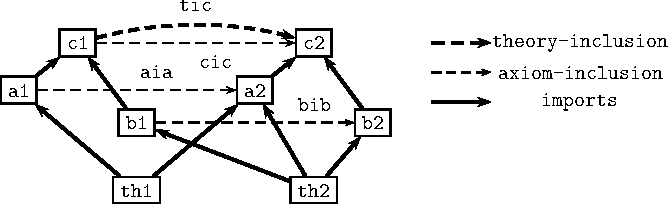
\includegraphics{pspic1.pdf}\else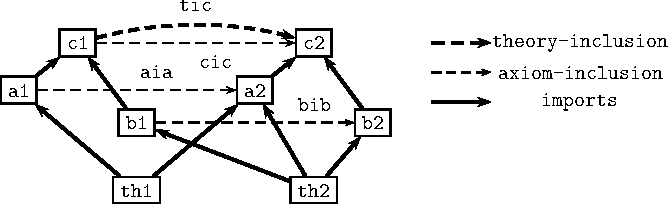
\includegraphics{pspic1.epsi}\fi
% exported to 
% \begin{pspicture}(-.5,-0.8)(11,2.7)
%   \rput(2,-0.5){\rnode{th1}{\psframebox{{\tt{th1}}}}}
%   \rput(5,-0.5){\rnode{th2}{\psframebox{{\tt{th2}}}}}
%   \rput(0,1.2){\rnode{a1}{\psframebox{{\tt{a1}}}}}
%   \rput(2,0.65){\rnode{b1}{\psframebox{{\tt{b1}}}}}
%   \rput(1,2){\rnode{c1}{\psframebox{{\tt{c1}}}}}
%   \rput(4,1.2){\rnode{a2}{\psframebox{{\tt{a2}}}}}
%   \rput(6,0.65){\rnode{b2}{\psframebox{{\tt{b2}}}}}
%   \rput(5,2){\rnode{c2}{\psframebox{{\tt{c2}}}}}

%   \ncline[linewidth=1.5pt]{->}{th1}{a1}\ncline[linewidth=1.5pt]{->}{th1}{a2}
%   \ncline[linewidth=1.5pt]{->}{th2}{b1}\ncline[linewidth=1.5pt]{->}{th2}{a2}\ncline[linewidth=1.5pt]{->}{th2}{b2}
%   \ncline[linewidth=1.5pt]{->}{a1}{c1}\ncline[linewidth=1.5pt]{->}{a2}{c2}
%   \ncline[linewidth=1.5pt]{->}{b1}{c1}\ncline[linewidth=1.5pt]{->}{b2}{c2}

%   \ncline[linestyle=dashed]{->}{a1}{a2}\aput(.6){{\tt{aia}}}
%   \ncline[linestyle=dashed]{->}{b1}{b2}\aput(.8){{\tt{bib}}}
%   \ncline[linestyle=dashed]{->}{c1}{c2}\bput(.6){{\tt{cic}}}
%   \ncarc[linestyle=dashed,arcangle=15,linewidth=1.5pt]{->}{c1}{c2}\aput(.5){{\tt{tic}}}
%   \rput(7,2){\pnode{ti1}}\rput(8,2){\pnode{ti2}}\ncline[linestyle=dashed,linewidth=1.5pt]{->}{ti1}{ti2}
%   \rput(9.5,2){{\element{theory-inclusion}}}
%   \rput(7,1.5){\pnode{ai1}}\rput(8,1.5){\pnode{ai2}}\ncline[linestyle=dashed]{->}{ai1}{ai2}
%   \rput(9.5,1.5){{\element{axiom-inclusion}}}
%   \rput(7,1){\pnode{ii1}}\rput(8,1){\pnode{ii2}}\ncline[linewidth=1.5pt]{->}{ii1}{ii2}
%   \rput(9.5,1){{\element{imports}}}
% \end{pspicture}
}\\[1ex]\baselineskip=8pt
\begin{boxedverbatim}
<theory id="th1">...</theory>     <theory id="th2">...</theory> 

<theory id="a1">                  <theory id="b1">
 <imports id="ima1" from="th1"/>   <imports id="imb1" from="th2"/>
 <axiom id="axa11"> ... </axiom>    <axiom id="axb1"> ... </axiom>
 <axiom id="axa12"> ... </axiom>   </theory>
</theory>

<theory id="a2">                  <theory id="b2">
 <imports id="im1a2" from="th1"/>  <imports id="imb2"a from="th2"/>
 <imports id="im2a2" from="th2"/> 
 <axiom id="axa2"> ... </axiom>    <axiom id="axb2"> ... </axiom>
</theory>                         </theory>

<theory id="c1">                  <theory id="c2">
 <imports id="im1c1" from="a1"/>  <imports id="im1c2"a from="a2"/>
 <imports id="im2c1" from="b1"/>  <imports id="im2c2"a from="b2"/>
 <axiom id="axc1"> ... </axiom>    <axiom id="axc1"> ... </axiom>
</theory>                          </theory>

<theory-inclusion id="tic" from="th1" to="th2"/>
<decomposition id="ti1d" for="ti1" links="aic bic cic"/>

<axiom-inclusion id="aic" from="a1" to="c2">
 <path-just local="aia" globals="im1c2"/>
</axiom-inclusion>

<axiom-inclusion id="bic" from="a1" to="c2">
 <path-just local="bib" globals="im2c2"/>
</axiom-inclusion>

<axiom-inclusion id="aia" from="a1" to="a2">
 <obligation induced-by="axa11" assertion="th-axa11"/>
 <obligation induced-by="axa12" assertion="th-axa12"/>
</axiom-inclusion>

<axiom-inclusion id="bib" from="b1" to="b2">
 <obligation induced-by="axb1" assertion="th-axb1"/>
</axiom-inclusion>

<axiom-inclusion id="cic" from="c1" to="c2">
 <obligation induced-by="axc1" assertion="th-axc1"/>
</axiom-inclusion>
\end{boxedverbatim}
\end{center}
\end{myfig}

\subsection{Parametric theories in {\ifpdf{OMDoc}\else{\omdoc}\fi}}\label{sec:parametric-theories}

Very often, the inheritence mechanisms presented so far do not suffice to model
mathematical practice, since they do not allow for parameterization. In
mathematics, the technique of studying certain aspects of complex mathematical
objects in isolation by factoring out the remaining objects into generic
parameters that can later be instantiated with concrete values is a key method for
reducing the complexity inherent in the reasoning process. The technique also
helps to modularize and reuse parts of specifications and theories. Before we
discuss the parameterization issues in {\omdoc} let us look at a concrete example:
a theory of lists of natural numbers.

We first specify a theory of lists that is generic in the elements, then we will
instantiate this by applying this theory to the special element theory of natural
numbers to obtain the intended theory of lists of natural numbers. The advantage
of this approach is that we can now re-use the generic theory of lists to apply it
to other element theories like that of sets of natural numbers to obtain a theory
of lists of sets of natural numbers.  In algebraic specification languages, we
speak of {\defemph{parametric theories}}\index{parametric
  theory}\index{theory!parametric}, i.e. the theory of lists has a formal
{\indextoo{parameter}} (in our example the set of elements) that can be
instantiated later with concrete values to get a {\defins{theory
    instance}}\index{instance!theory} (in our example the theory of lists of
natural numbers). We call this process theory {\indextoo{actualization}}.

\begin{myfig}{actualization}{A Structured Specification of Lists}
\begin{center}
\fbox{\ifpdf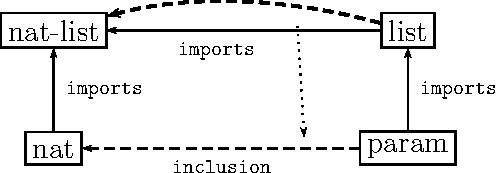
\includegraphics{pspic2.pdf}\else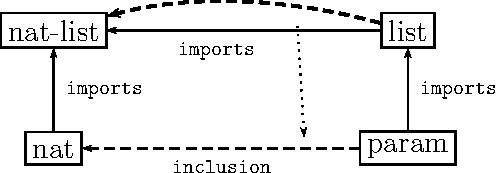
\includegraphics{pspic2.epsi}\fi
% \psset{unit=2cm}
%   \begin{pspicture}(-1.6,-0.2)(3,1.4)
%     \rput(-1,0){\rnode{nat}{\psframebox{{\Large nat}}}}
%     \rput(2,0){\rnode{elt}{\psframebox{{\Large param}}}}
%     \rput(-1,1){\rnode{natlist}{\psframebox{{\Large nat-list}}}}
%     \rput(2,1){\rnode{list}{\psframebox{{\Large list}}}}
%     \ncline[linestyle=dashed]{->}{elt}{nat}\aput(.5){{\tt{inclusion}}}\bput(.2){\pnode{dectarget}}
%     \ncline{->}{nat}{natlist}\bput(.5){{\tt{imports}}}
%     \ncline{->}{list}{natlist}\aput(.6){{\tt{imports}}}
%     \ncline{->}{elt}{list}\bput(.5){{\tt{imports}}}
%     \ncarc[arcangle=15,linestyle=dashed,linewidth=1.5pt]{<-}{natlist}{list}\bput(.7){\pnode{decsource}}
%     \ncline[nodesep=0pt,linestyle=dotted]{->}{decsource}{dectarget}
%   \end{pspicture}
}\\[1ex]\baselineskip=8pt\scriptsize
\begin{boxedverbatim}
<theory id="param">                   
 <symbol id="elem" type="sort"/>       
 <symbol id="ord"/>
 <axiom id="toset"><CMP>\(ord\) is a  total order on \(elem\).</CMP></axiom>
</theory>                               
                                       
<assertion id="ord-nat" theory="nat"> 
 <CMP>\(geq\) is a total order on \(nats\).<OMOBJ>.
 </CMP>
<assertion>

<theory id="list">
 <imports id="list.im" from="param"/>
 <symbol id="list-sort" type="sort"/>
 <symbol id="cons"/><symbol id="nil"/>
 <symbol id="ordered"/>
</theory>

<theory id="nat-list">
 <imports id="nat-list.im-nat" from="nat"/>
 <imports id="nat-list.im-elt" from="list" type="local">
  <morphism id="elem-nat">
   <requation>
    <pattern><OMOBJ><OMS cd="param" name="elem"/></OMOBJ></pattern>
    <value><OMOBJ><OMS cd="nat.thy" name="nats"/></OMOBJ></value>
   </requation>
  </morphism>
 </imports>
 <inclusion via="elem-nat-incl"/>
</theory>

<axiom-inclusion id="elem-nat-incl" from="nat" to="param">
 <morphism id="elem-nat-incl-morph" base="elem-nat"/>
 <obligation induced-by="toset" assertion="ord-nat"/>
</axiom-inclusion>

<theory-inclusion id="nat-natlist-incl" from="list" to="nat-list">
 <morphism id="nat-natlist-incl-morph" base="elem-nat"/>
</theory-inclusion>
<decomposition id="dec" for="nat-natlist-incl" links="elem-nat-incl"/>
\end{boxedverbatim}
\end{center}
\end{myfig}

Parts of this process can be modeled in the {\omdoc} development graph model of theory
inheritance by constructing dedicated parameter theories. Consider the situation in
{\myfigref{actualization}}, where we have theories {\ttin{nat}} of natural numbers (for
instance one that contains the abstract data type in {\myfigref{nat-adt}}) and a generic
theory {\ttin{list}} of lists that imports its elements from a generic parameter theory
{\ttin{param}}.  There the theory {\ttin{nat-list}} of lists of natural numbers is built
up by importing from the theories {\ttin{nat}} and {\ttin{list}} making the {\tt{nat}} the
actual parameter theory in the process. Note that the attribute
{\attribute{type}{imports}} of the {\element{imports}} element {\tt{nat-list.im-elt}} is
set to {\attval{local}{type}{imports}}, since we do not want to import the local axioms of
the theory {\tt{list}} and not the whole theory {\tt{list}} (which would include the
axioms from {\tt{param}}).  The effect of the actualization comes from the morphism
{\tt{elem-nat}} in the import of {\ttin{List}} that renames the symbol {\tt{elem}} (from
theory {\tt{param}}) with {\tt{nats}} (from theory {\tt{nat}}).

Note that this naive encoding of actualization does not always lead to the
expected result that there is a theory inclusion from the theory {\tt{list}} to
{\tt{nat-list}}. Say we are actually trying to specify a theory of
{\indextoo{ordered lists}}\index{list!ordered}, then we need an ordering relation
on the set {\tt{elem}} of elements. We introduce a symbol {\tt{ord}} and the
necessary axiom in the theory {\tt{param}} to make {\tt{elem}} a totally ordered
set. As {\tt{param}} is imported into {\tt{list}}, these are available to specify
ordered lists in the theory {\tt{list}}. Now, if we do the actualization from
{\tt{List}} to {\tt{nat-list}}, we have to ensure that the parameter theory
{\tt{nat}} also has a suitable ordering function. This can be specified using the
{\omdoc} {\element{inclusion}} element.  {\eldef{inclusion}} is an empty element
whose {\attribute{via}{inclusion}} attribute points to an axiom inclusion from the
generic parameter theory to the actual parameter theory whose morphism extends the
import morphism of the parameter theory. In our examples we can see that the
{\element{axiom-inclusion}} specified in the {\element{inclusion}} element is
sufficient to guarantee the theory inclusion from {\tt{nat}} to {\tt{nat-list}}
that states the correctness of the parameter actualization. For more details
see~\cite{Hutter:mocsv00}.

Note that this mechanism for parametric theories only works in situations with an
a-priori finite number of possible theory instances, since these have to be
explicitly generated in advance. However theorem provers like the {\pvs}
system~\cite{OwRu92} also allow to quantify over variables that are later used to
instantiate theory parameters; in this case the number of theory instances is
potentially infinite, and cannot be directly be represented in {\omdoc}.
Unfortunately this problem cannot simply be fixed by adding additional
representation concepts to {\omdoc}, since it breaks a fundamental assumption in
{\openmath}, namely that theories can always explicitly be represented (as content
dictionaries), and that this can be done ahead of using them. Thus extending
{\mbase}/{\omdoc} to this form of mathematical practice will reconciling even
something as fundamental as the {\openmath} standard with mathematical practice.
Note that the concept of parametric theories cannot easily be dismissed as
representational aberrations; the work on so-called functors in the Theorema
project {\url{http://www.theorema.org}} views parametric theories as the principal
building blocks and successfully uses this higher-order structure to guide theorem
proving.

\section{Auxiliary Elements}\label{sec:auxitems}

Up to now, we have been mainly concerned with providing elements for marking up
the inherent structure of mathematical knowledge in mathematical statements and
theories. We have not bothered yet about representing the structure of
mathematical documents themselves (as structured text entities), or the
information that is necessary transforming the mathematics into formats suitable
for communicating with humans or mathematical software systems. We will introduce
the necessary infrastructure in this section.

In~\ref{sec:text-structure} we will present {\omdoc} elements for representing the
text structure of mathematical documents as structured text entities. This makes
it possible to transform legacy documents into {\omdoc} form without losing
information: the paragraphs of the input document are classified into mathematical
statements wherever possible and the remaining are represented as
{\element{omtext}}. The text structure of the input document (paragraphs, sections,
and chapters) is represented by {\element{omgroup}} elements of suitable types;
some of these may also be reflected in the theory structure organizing the
knowledge.

In~\ref{sec:private} we introduce an infrastructure for interfacing {\omdoc}
documents with the Internet in general and mathematical software systems in
particular. The application of this is that we can generate representations from
{\omdoc} documents where formulae, statements or even theories that are active
components that can directly be manipulated by the user or mathematical software
systems.

Finally, we present a present a limited infrastructure for mathematical exercises
in section~\ref{sec:exercises}. This allows to use {\omdoc} as a basis for
mathematical education and assessment. Note that the infrastructure introduced
here is relatively little developed, and born out of the immediate need of
{\omdoc} projects. We envision that in the future we will use specialized {\xml}
vocabularies like the IMS standard for questions and
exercises~\cite{SmyShe:iqti01}.

\subsection{Preservation of Text Structure}\label{sec:text-structure}

Like other documents, mathematical ones are often divided into units like
chapters, sections, and paragraphs by tags and nesting information. {\omdoc} makes
these document relations explicit with specialized {\element{omgroup}} elements.
These have an attribute {\attribute{type}{omgroup}} that can take values including
{\attval{item\-ize}{type}{omgroup}}, {\attval{sequence}{type}{omgroup}},
{\attval{enumerate}{type}{omgroup}} with the obvious meanings as text groups. The
{\attribute{type}{omgroup}} attribute can be used to specify other grouping
devices, such as {\attval{dataset}{type}{omgroup}} for table and
{\attval{theory-collection}{type}{omgroup}}, which we will discuss elsewhere in
this document (consult the attribute table on in appendix~\ref{sec:att-table}).

We consider the {\element{omdoc}} element as an implicit {\element{omgroup}}, in
order to allow plugging together different different {\omdoc} documents as
{\element{omgroup}s}. As a consequence, the {\element{omdoc}} element has also has
an {\attribute{type}{omdoc}} attribute that can take the same values as that for
the {\element{omgroup}} element. {\element{omgroup}} elements can appear at
{\indextoo{top-level}}, and can contain any top-level elements. As the document
structure need not be a tree in hypertext documents, {\eldef{omgroup}} elements
also allow {\eldef{ref}} elements whose {\attribute{xref}{ref}} attribute can be
used to reference {\omdoc} elements defined elsewhere. The {\attribute{type}{ref}}
attribute can be used to describe the reference type. Currently {\omdoc} supports
two values: {\attval{include}{type}{ref}} (the default) for in-text replacement
and {\attval{cite}{type}{ref}} for a proper reference. The first kind of reference
requires the {\omdoc} application to process the document as if the
{\element{ref}} element were replaced with the {\omdoc} fragment specified in the
{\attribute{xref}{ref}}. The processing of the second type is application specific
it is recommended to generated an appropriate label and (optionally) supply a
hyper-reference. There may be more supported values for {\attribute{type}{ref}} in
time.

This structuring approach allows to ``{\indextoo{flatten}}'' the tree structure in
a document into a list of leaves and relation declarations (see
{\myfigref{flatten}} for an example). It also makes it possible to have more than
one ``view'' on a document using {\element{omgroup}} structures that reference to
a shared set of {\omdoc} elements as leaves.

\setbox0=\hbox{\begin{minipage}{4.5cm}\scriptsize
\begin{alltt}
<omgroup id="text" 
         type="sequence">
 <omtext id="t1">{\rm{T1}}</omtext>
 <omgroup id="enum" 
          type="enumeration">
  <omtext id="t2">{\rm{T2}}</omtext>
  <omtext id="t3">{\rm{T3}}</omtext>
 </omgroup>
 <omtext id="t4">{\rm{T4}}</omtext>
</omgroup>
\end{alltt}
\end{minipage}}
\setbox1=\hbox{\begin{minipage}{5.6cm}\scriptsize
\begin{alltt}
<omtext id="t1">{\rm{T1}}</omtext>
<omtext id="t2">{\rm{T2}}</omtext>
<omtext id="t3">{\rm{T3}}</omtext>
<omtext id="t4">{\rm{T4}}</omtext>

<omgroup id="text" type="sequence">
  <ref xref="t1"/>
  <ref xref="enum"/>
  <ref xref="t4"/>
</omgroup>

<omgroup id="enum" type="enumeration">
  <ref xref="t2"/>
  <ref xref="t3"/>
</omgroup>
\end{alltt}
\end{minipage}}
\begin{myfig}{flatten}{Flattening a tree structure}
\fbox{\box0}$\;\longleftrightarrow\;$\fbox{\box1}
\end{myfig}

While the {\omdoc} approach to specifying document structure is a much more
flexible (database-like) approach to representing structured
documents\footnote{The simple tree model is sufficient for simple markup of
  existing mathematical texts and to replay them verbatim in a browser, but is
  insufficient e.g. for generating individualized presentations at multiple levels
  of abstractions from the representation. The {\omdoc} text model -- if taken to
  its extreme -- allows to specify the respective role and contributions of
  smaller text units, even down to the sub-sentence level, and make the structure
  of mathematical texts ``machine understandable''. Thus, an advanced presentation
  engine like the {\activemath} system~\cite{SieBen:acgap00} can -- for instance
  -- extract document fragments based on the preferences of the respective user.},
than the tree model, it puts a much heavier load on a system for presenting the
text to humans. In essence the presentation system must be able to recover the
left representation from the right one in {\myfigref{flatten}}. Generally, any
{\omdoc} element defines a fragment of the {\omdoc} it is contained in: everything
that this element contains and (recursively) those elements that are reached from
it by following the cross-references. In particular, the text fragment
corresponding to the element with ({\attribute{id}{omtext}}={\tt{"text"}}) in the
right {\omdoc} of~\myfigref{flatten} is just the one on the right.

\begin{myfig}{qtgeneral}{{\omdoc} elements for specifying  document structure.}
  \quicktable{\generaltable{}}
\end{myfig}

The {\element{omgroup}} element has other uses in {\omdoc}, it can be used specify
{\indextoo{data set}s}, a content-oriented generalization of {\indextoo{table}s}
to arbitrary dimensions. {\omdoc} views tables as instances of sets of data
structured into $k$ dimensions and reserves the value
{\attval{dataset}{type}{omgroup}} for this purpose. Conventional tables are just
the two-dimensional special case.

\begin{myfig}{table}{Specifying Tables with {\tt{<omgroup type="dataset">}}}
  \begin{tabular}{l|lll}
    name &  a1  & a2  & a3\\\hline
    b1  &  e11  & e12 & e13\\         
    b2  &  e21  & e22 & e23\\
  \end{tabular}\\
\begin{scriptsize}
\begin{boxedverbatim}
<omgroup id="example-table" type="labeled-dataset">
 <metadata><Title>name</Title></metadata>

 <omgroup id="f1" type="dataset">
  <omgroup type="dataset"><omtext><CMP>a1</CMP></omtext></omgroup>
  <omgroup type="dataset"><omtext><CMP>a2</CMP></omtext></omgroup>
  <omgroup type="dataset"><omtext><CMP>a3</CMP></omtext></omgroup>
 </omgroup>

 <omgroup id="f2" type="dataset">
  <omgroup type="dataset"><omtext><CMP>b1</CMP></omtext></omgroup>
  <omgroup type="dataset"><omtext><CMP>b2</CMP></omtext></omgroup>
 </omgroup>

 <omgroup id="data" type="dataset">
  <omgroup id="dc1" type="dataset">
   <omgroup type="dataset"><omtext><CMP>e11</CMP></omtext></omgroup>
   <omgroup type="dataset"><omtext><CMP>e12</CMP></omtext></omgroup>
   <omgroup type="dataset"><omtext><CMP>e13</CMP></omtext></omgroup>
  </omgroup>
  
  <omgroup id="dc2" type="dataset">
   <omgroup type="dataset"><omtext><CMP>e21</CMP></omtext></omgroup>
   <omgroup type="dataset"><omtext><CMP>e22</CMP></omtext></omgroup>
   <omgroup type="dataset"><omtext><CMP>e23</CMP></omtext></omgroup>
  </omgroup>
 </omgroup>
</omgroup>
\end{boxedverbatim}
\end{scriptsize}
\end{myfig}
Let us analyze this approach using the example in {\myfigref{table}}, which is a
$k=2$-dimensional special case. The $n=2\times m=3$-table in the top is modeled as the
outer {\element{omgroup}} element, the value {\attval{labeled-dataset}{type}{omgroup}}
signifies that this is a table where the axes are labeled. The name of the table can be
given in the {\element{metadata}}/{\element{Title}}. The outer {\element{omgroup}} element
organizes the table information into two parts. The first part (the first $k$ elements)
contains the label information and the last element the data proper. All of these elements
are {\element{omgroup}s} of type {\attval{dataset}{type}{omgroup}}, which signifies that
they do not contain label information.  The nesting depth of the {\element{omgroup}}
elements corresponds to the dimension of the data sets involved. The $k$ label elements
are $k-1=1$-dimensional data sets in our example, while the body is $k=2$-dimensional, and
is organized into $n=2$ rows, which again are {\element{omgroup}s} of
{\attribute{type}{omgroup}} {\attval{dataset}{type}{omgroup}} (one-dimensional tables).
The generalization for higher dimensions is obvious (e.g. for a $k=3$-dimensional $l\times
n\times m$-array we would have an {\element{omgroup}} that has a $n\times m$-table of
labels like the one in {\myfigref{table}}, followed $k$ such {\element{omgroup}} elements
for the $k$ levels). Note that the final table entries are modeled as $0$-dimensional data
sets, and thus contain a seemingly spurious {\element{omgroup}}. This makes the approach
more flexible (we can have structured text objects in table entries) and more uniform (and
thus entails better substitution properties).

This content-based approach makes the components of tables more explicit than
presentation-based ones. In particular, we can reference individual parts like rows and
columns by their {\attribute{id}{omgroup}} attributes for later reference. We can also add
metadata to sub-structures like labeling of faces of the tables, e.g. the face {\tt{f2}}
could have a {\element{metadata}} element with a {\element{Description}} that says that
the data are temperatures in degree Celsius.

Of course, the {\attval{dataset}{type}{omgroup}} {\element{omgroup}s} only specify the
content of the tables, the concrete appearance in the output format generated will be
determined by a presentation component.

\subsection{Non-{\ifpdf{XML}\else{\xml}\fi} Data and Program Code in {\ifpdf{OMDoc}\else{\omdoc}\fi}}\label{sec:private}

\begin{myfig}{qtcode}{The {\omdoc} Auxiliary Elements for non-{\xml} Data}
  \quicktable{\omlettable{}}
\end{myfig}
The {\omdoc} elements we have presented standardize the representation of general
mathematical knowledge. Since we have taken care to allow the formal representation
of mathematical objects at every level, this is a representational infrastructure
that is sufficient as an output and library format for mathematical software
systems like computer algebra systems, theorem provers, or theory development
systems. In particular, having a standardized output and and library format will
enhance system interoperability, and allows to build and deploy general storage
and library management systems like {\mbase} (see~\ref{sec:mbase}).

However, most mathematical software systems need to store and communicate data,
which is system-specific, but may be relevant to more than user. Examples of this
are pieces of {\edin{program}} code, like tactics or proof search heuristic of
tactical theorem provers or linguistic data of proof presentation systems. Only if
these data can be integrated into {\omdoc}, will it become a full storage and
communication format for mathematical software systems. One characteristic of such
system-specific data is that it is often not in {\xml} syntax, or its
format is  not  fixed enough to warrant for a general {\xml} encoding. 

For this kind of data, {\omdoc} provides the {\element{private}} and
{\element{code}} elements. Their attributes contain metadata information
identifying system requirements and relations to other {\omdoc} elements. We will
first describe the shared attributes and then describe the elements themselves.
\begin{description}
\item[{\attribute{id}{private, code}}] (required) for identification.
\item[{\attribute{theory}{private, code}}] this optional attribute allows the
  specification of the mathematical theory (see section~\ref{sec:theories}) that
  the data is associated with.
\item[{\attribute{for}{private, code}}] which allows to attach the data to some
  other {\omdoc} element. Attaching {\element{private}} elements to {\omdoc}
  elements is the main mechanism for system-specific extension of {\omdoc}.
\item[{\attribute{pto}{private, code}}] is a whitespace-separated list of token names
  which specifies the set of systems to which the data are private. The intention
  of this field is that a {\element{private}} element is visible to all systems,
  but should only manipulated by a system that are mentioned here.
\item[{\attribute{pto-version}{private, code}}] is a whitespace-separated list of tokens
  for version numbers; This only makes sense, if the value of the corresponding
  {\attribute{pto}{private, code}} is a singleton. Specifying this may be necessary, if
  the data or even their format change with versions.
\item[{\attribute{type}{private, code}}] the type of the data, the meaning of these
  fields is determined by the system itself. 
\item[{\attribute{requires}{private, code}}] specifies the identifiers of the
  elements that the data depend upon, which will often be {\element{code}}
  elements. This allows to factor private data into smaller parts, allowing more
  flexible data storage and retrieval. This is especially interesting for program
  code or private data that relies on program code. This can broken up into
  procedures and the call-hierarchy can be encoded in
  {\attribute{requires}{private, code}} attributes. Based on this information, a
  storage application based on {\omdoc} can then always communicate a minimal
  complete code set to the requesting application.
\end{description}

The {\eldef{private}} element is intended for system-specific data that is not
program code. It contains a {\element{metadata}} element and a set of
{\element{data}} elements that contain or reference the actual data. The
{\element{private}} element adds the {\attribute{replaces}{private}} attribute to
those described above. This specifies the identifiers (given in the
{\attribute{id}{private, code}} attribute) of {\omdoc} elements that are subsumed
by the information in the private element. A special case is the empty private
element (empty {\element{data}} element), that can be used to specify that certain
{\omdoc} elements are irrelevant to a given application.

The {\eldef{data}} element contains the data in a {\ttin{CDATA}} section.  It has
the attribute {\attribute{format}{data}} to specify the format the data are in,
e.g.  {\ttin{image/jpeg}} or {\ttin{image/gif}} for image data, {\ttin{binary}}
for system-specific binary data, {\ttin{text/plain}} for text data, etc. It is
good practice to use the {\indextoo{MIME}} types for this purpose, wherever
applicable. In a {\element{private}} or {\element{code}} element, the
{\element{data}} elements must differ in their {\attribute{format}{data}}
attribute. If the content of this field is too large to store directly in the
{\omdoc} or changes often, then it can be substituted by a link, specified in the
{\attribute{href}{data}} attribute. The optional {\attribute{size}{data}}
attribute can be used to specify the size of the outside resource.

The {\eldef{code}} element is used for embedding pieces of program code into an
{\omdoc} document. This element has the attributes described above plus attributes
{\attribute{codebase}{private}} and {\attribute{classid}{private}}, if it contains
{\indextoo{Java}} code. It contains the documentation elements {\eldef{input}},
{\eldef{output}}, and {\eldef{effect}} that specify the behavior of the procedure
defined by the code fragment. The {\element{input}} element describes the
structure and scope of the input arguments, {\element{output}} the outputs
produced on these elements, and {\element{effect}} any side effects the procedure
may have.  They contain a multilingual {\element{CMP}} elements with an optional
{\element{FMP}} for a formal description. The latter may be used for program
verification purposes. If any of these elements are missing it means that we may
not make any assumptions about them, not that there are no inputs, outputs or
effects. For instance, to specify that a procedure has no side-effects we need to
specify something like {\tt{<effect><CMP>None.</CMP></effect>}}. These elements
are followed by a set of {\element{data}} elements that contain or cross-reference
the program code itself. {\Myfigref{omlet1}} shows an example of a
{\element{code}} element used to store {\indextoo{Java}} code for an applet.

\subsection{Applets in {\ifpdf{OMDoc}\else{\omdoc}\fi}}\label{sec:applets}

Web-based text markup formats like {\html} have a concept of an
{\indextoo{applet}}, i.e.  programs that can in some way executed in the browser
during document manipulation. This one of the primary ways used to enliven parts
of the document.
\begin{myfig}{link}{Some hyperlinks an {\element{omlet}}.}\scriptsize
\begin{boxedverbatim}
<CMP>The missing parts are 
 <omlet type="link" argstr="file://missing.html">here (html)</omlet>.
  For the mathematical background see
 <omlet type="preslink" argstr="file://back.omdoc">this</omlet>.
</CMP>
\end{boxedverbatim}
\end{myfig}

In {\omdoc}, we use the {\eldef{omlet}} element for applets and generalizes the
{\indextoo{applet}} concept in two ways: The computational engine is not
restricted to {\indextoo{plug-in}s} of the browser and the program code can be
included in the {\omdoc} document, making document-centered computation easier to
manage. 

The simplest application of {\element{omlet}} elements is the specification of
hyperlinks. {\Myfigref{link}} shows two. The first one is a very simple hyperlink
to a {\html} file, the second one is a hyperlink to an {\omdoc} document, that
will have to be translated into the current presentation format before it can be
viewed by the user. Since hyperlinks are so important in mathematical documents,
we reserve the keywords {\attval{link}{type}{omlet}} and
{\attval{preslink}{type}{omlet}} for hyperlinks. Note that even for such a simple
case as hyperlinks, the differences between hyperlinks and applets are blurred,
therefore {\omdoc} only provides the {\element{omlet}} element for both.

\setbox0=\hbox{\footnotesize\begin{minipage}{11cm}
\begin{alltt} 
<code id="callMint" codebase="org.riaca.cas"> 
 <CMP>
  The multiple integrator applet. It puts up a user interface 
  queries the user for a function, which it then integrates 
  by calling one of several computer algebra systems. 
 </CMP>
 <input>None, the applet handles input itself.</input> 
 <output>The result of the integration.</output>
 <effect>None.</effect> 
 <data format="java">
  <![CDATA[... {\em the callMint code goes here} ...]]>
 </data> 
</code>

<omtext id="monp_1">    
 <CMP> Let's <omlet type="js" function="callMint" action="execute">
     Integrate</omlet>!
 </CMP>
</omtext>
\end{alltt}\end{minipage}}
\begin{myfig}{omlet1}{An {\element{omlet}} that calls a Java applet.}
   \fbox{\box0}
\end{myfig}
Like the {\html} {\ttin{applet}} tag, the {\element{omlet}} element can be used to wrap any
(set of) well-formed element. It has the following attributes. 
\begin{description}
\item[{\attribute{type}{omlet}}] This specifies the computation engine that should
  execute the code. Depending on the application, this can be a programming
  language, such as {\tt{javascript}} ({\attval{js}{type}{omlet}}) or {\oz}, or a
  process that is running, e.g. a theorem prover.
\item[{\attribute{function}{omlet}}] The code that should be executed by the omlet is
  specified in the {\attribute{function}{omlet}} attribute. This points to an {\omdoc} code
  element that is somehow accessible (e.g. in the same {\omdoc}). This
  indirection allows us to reuse the machinery for storing code in {\omdoc}s. For
  a simple example see {\myfigref{omlet1}}. 
\item[{\attribute{argstr}{omlet}}] This optional attribute allows to specify an
  argument string for the function called by the applet, so that the program in
  the can be kept general. A call to the {\loui} interface, would for example have
  the form in {\myfigref{omlet2}}.  Here, the code in the {\element{code}} element
  {\tt{sendtoloui}} (which we have not shown) would be Java code that simply sends
  the value of the {\attribute{argstr}{omlet}} to {\loui}'s remote control port.
\item[{\attribute{width}{omlet}}/{\attribute{height}{omlet}}] gives the screen
  height and width of the applet.
\end{description}
The expected behavior of the {\element{omlet}} can be implemented in the {\xslt}
style sheet, that in the case of e.g. translation to {\mozilla} will put the
{\ttin{callMint}} code directly into the generated {\ttin{html}}.
\setbox0=\hbox{\footnotesize\begin{minipage}{8.6cm}\begin{alltt}
<CMP> Let's prove it 
  <omlet id="bla" type="java" function="sendtotp"
         argstr="load(problem='monoid_uniq')">
    interactively
  </omlet>. 
</CMP>
\end{alltt}\end{minipage}}
\begin{myfig}{omlet2}{An {\element{omlet}} for connecting to a theorem prover.}
  \fbox{\box0}
\end{myfig}

\subsection{Exercises}\label{sec:exercises}

Exercises are vital parts of mathematical textbooks.  In {\omdoc}, we use the
{\eldef{exercise}} element for representing them. The question statement is
represented in the multilingual {\element{CMP}} group followed by an optional
{\element{FMP}} element and an optional {\eldef{hint}} element that contains a
hint in a {\element{CMP}}/{\element{FMP}} group.

\begin{myfig}{qtex}{The {\omdoc} Auxiliary Elements for Exercises}
  \quicktable{\extable{}}
\end{myfig}

The next element in an {\element{exercise}} is either a (set of) possible
solutions, or a multiple-choice block. The first is represented in a
{\eldef{solution}} element with a a {\element{CMP}}/{\element{FMP}} group followed
by an optional {\element{proof}} or {\element{proofobject}}. A special case of
this is the case, where the question contains an assertion whose proof is not
displayed and left to the reader. In this case, the {\element{solution}} contains
a proof.  {\indextoo{Multiple-choice exercise}s} (see {\myfigref{exercise}}) are
represented by a list of {\eldef{mc}} elements.  These represent a single choice
in a {\eldef{choice}} element together with the answer in the {\eldef{answer}}
element.  The {\attribute{verdict}{answer}} of the {\element{answer}} element
attribute specifies the truth of the answer, it can have the values
{\attval{true}{verdict}{answer}} or {\attval{false}{verdict}{answer}}.  The
{\element{choice}} and {\element{answer}} elements contain
{\element{CMP}}/{\element{FMP}} groups.

\setbox0=\hbox{\footnotesize\begin{minipage}{11.8cm}\begin{alltt}
<exercise for="ida.c6s1p4.l1" id="ida.c6s1p4.mc1">
 <CMP>What is the unit element of the semi-group \(Q\)
  with operation \(a*b = 3ab\)?
 </CMP> 
 <mc><choice><FMP><OMOBJ><OMI>1</OMI></OMOBJ></FMP></choice>
     <answer verdict="false"><CMP>No, \(1*1=3\) and not 1</CMP></answer>
 </mc>
 <mc><choice><CMP>1/3</CMP></choice>
     <answer verdict="true"></answer>
 </mc>
 <mc><choice><CMP>It has no unit.</CMP></choice>
     <answer verdict="false"><CMP>No, try another answer</CMP></answer>
 </mc>
</exercise>
\end{alltt}\end{minipage}}  
\begin{myfig}{exercise}{An Exercise}
   \fbox{\box0}
\end{myfig}


\section{Adding Presentation Information to {\ifpdf{OMDoc}\else{\omdoc}\fi}}

As we have seen, {\omdoc} is concerned mainly with the content and structure of
mathematical documents, and offers a complex infrastructure for dealing with that.
However, mathematical texts often carry typographic conventions that
cannot be determined by general principles alone. Moreover, non-standard
presentations of fragments of mathematical texts sometime carry meanings that do
not correspond to the mathematical content or structure proper. In order to
accomodate this, {\omdoc} provides a limited functionality for embedding style
information into the document.

The normal (but of course not the only) way to generate presentation from {\xml}
documents is to use {\xslt} style sheets (see section~\ref{sec:transform-xsl} for
other applications).  {\xslt}~\cite{Deach:exls99} is a general transformation
language for {\xml}.  {\xslt} programs (often called {\indextoo{style sheet}s})
consist of a set of so-called {\indextoo{templates}} (rules for the transformation
of certain nodes in the {\xml} tree). These templates are recursively applied to
the input tree to produce the desired output.

The general approach is not to provide general-purpose presentational primitives
that can be sprinkled over the document, since that would distract the author from
the mathematical content, but to support the specification of general style
information for {\omdoc} elements and mathematical symbols in separate elements.

In the case of a single {\omdoc} document it is possible to write a specialized
style sheet that transforms the content-oriented markup used in the document into
mathematical notation. However, if we have to deal with a large collection of
{\omdoc} representations, then we can either write a specialized style sheet for
each document (this is clearly infeasible to do by hand), or we can develop a
style sheet for the whole collection (such style sheets tend to get large and
unmanageable).

{\omdoc} supports variants of both approaches, it allows to generate specialized
style sheets that are tailored to the presentation of (collections of) {\omdoc}
documents. The mechanism will be discussed in section~\ref{sec:transform-xsl},
here we only concern ourselves with the {\omdoc} primitives for representing the
necessary data. In the next subsection, we will address the specification of style
information for {\omdoc} elements by {\element{omstyle}} elements, and then the
question of specification of notation of mathematical symbols in
{\element{presentation}} elements.

\subsection{Specifying Style Information for {\ifpdf{OMDoc}\else{\omdoc}\fi} Elements}

{\omdoc} provides the {\eldef{omstyle}} elements for specifying {\indextoo{style
    information}}\index{information!style} for {\omdoc} elements.  An
{\element{omstyle}} element has the attributes has the attributes
\begin{description}
\item[{\attribute{element}{omstyle}}] this required attribute specifies the
  {\omdoc} element this style information should be applied to. Note that the
  value of this attribute must be the full {\indextoo{qualified
      name}}\index{name!qualified} (i.e. including the {\index{namespace}}) of the
  element.
\item[{\attribute{for}{omstyle, presentation}}] this optional attribute allows to further
  restrict the {\omdoc} element to a single instance.
\item[{\attribute{xref}{omstyle, presentation}}] This optional attribute can be used to
  refer to another existing {\element{omstyle}} element (in another document),
  sometimes avoiding double specification.
\item[{\attribute{style}{omstyle, presentation}}] This optional attribute is is an
  additional parameter that controls the output style. This allows to specify
  different notational conventions for symbols. This attribute corresponds to the
  optional {\attribute{style}{*}} attributes in those {\omdoc} elements that have
  {\attribute{id}{*}} attributes. They can be used to specify the style intended
  by the document author and help choose a {\element{presentation}} element.
  
  Note that the choice of notational style is not a content-carrying feature, and
  should not be depended on, indeed the value of the
  {\attribute{stlye}{presentation}} need not be respected by output routines, but
  can be overwritten.
\end{description}
The information specified in the body of this element is then used to generate
{\xslt} templates that can be used in the style sheets. This information is either
given directly as the bodies of {\xslt} templates in the {\eldef{xslt}} element,
or in a {\eldef{style}} element using a small subset of {\xslt} internalized into
{\omdoc}. This second language is used if the full power of {\xslt} is not needed,
and has the advantage that it can be transformed into the input of other
formatting engines. The {\element{xslt}} and {\element{style}} elements share the
following attributes
\begin{description}
\item[{\attribute{format}{use, xslt, style}}] this required attribute specifies the output
  format. Its value is a string of format specifiers divided by the {\tt{|}}
  character. We use the specifiers {\attval{TeX}{format}{use}} for {\TeX} and
  {\LaTeX}, {\attval{pmml}{format}{use}} for presentation {\mathml},
  {\attval{cmml}{format}{use}} for content {\mathml}, {\attval{html}{format}{use}}
  for {\html}, {\attval{mathematica}{format}{use}} for {\mathematica} notebooks.
  Finally, there is the pseudo format-specifier {\attval{default}{format}{use}},
  which will be taken, if no other format is defined. Note that case matters in
  these specifiers, so {\tt{TeX}} is not the same as {\tt{tex}}, furthermore,
  {\attval{default}{format}{use}} is not a regular format specifier, so it cannot
  appear in the disjunctions.
  
  See {\url{http://www.mathweb.org/omdoc/xsl.html}} for other available formats.
  Similarly, the English language serves as a default language.
\item[{\attribute{xml:lang}{use, xslt, style}}] this specifies the language for
  which this notation is used. In contrast to the other uses of
  {\attribute{xml:lang}{use, xslt, style}} does not have a default value {\tt{en}}.
  If the attribute is not present, this means that this element is not
  language-specific.
\item[{\attribute{requires}{use, xslt, style}}] This attribute points to a {\element{code}}
  element that contains a code fragment that is needed to be included for the
  presentation engine. For instance, a {\element{use}} element for the format
  {\LaTeX} may contain macro calls that need to be defined. Their definitions
  would need to be included in the output document by the presentation style sheet
  before they can be used.
\end{description}

{\Myfigref{with}} shows very simple example, where a {\element{with}} element is
used to mark a text passage as ``important''. This style attribute is then picked
up in the {\element{omstyle}} element to prompt special treatment in the output.
Note that here the attributes of the {\element{use}} element are used to specify
bracketings, the presentation specified in the attributes are placed where the
{\xml} tags {\tt{<with>}} and {\tt{</with>}} are.

\begin{myfig}{with}{Specifying Style information with the {\element{with}}
    Element.}\footnotesize
\begin{boxedverbatim}
<CMP>
  I want to mark <with id="w1" style="important">this important
  text</with> as special.<with style="linebreak"/>
  I can also refer to 
  <with style="link"><OMOBJ><OMSTR>missing.html</OMSTR></OMOBJ>
   here</with>, if something is missing.
</CMP>

<omstyle element="omdoc:with" style="important">
  <style format='html|pmml'><element name="em"><recurse/></element></style>
  <xslt format='TeX'><[CDATA[{\em<xsl:apply-templates/>}]]></xslt>
</omstyle>

<omstyle element="omdoc:with" style="linebreak">
  <style format='html|pmml'><element name="br"/></style>
  <style format='TeX'><text>\par\noindent</text></style>
</omstyle>

<omstyle element="omdoc:with" style="link">
 <style format="html|pmml">
  <element name="a">
   <attribute name="href">
    <value-of select="om:OMOBJ/om:OMSTR"/>
   </attribute>
   <recurse select="*[not(om:OMOBJ)]/>
  </element>
 </style>
</omstyle>
\end{boxedverbatim}
\end{myfig}
Let us now look at the sub-language used in {\element{style}} elements.  We can
see in the second {\element{omstyle}} element that the content of the
{\element{xslt}} element are {\xslt} fragments. They have to be either enclosed in
a {\indextoo{CDATA}} section, of escaped. Note that when referring to {\omdoc}
elements, the {\xslt} must use the full {\indextoo{qualified
    name}}\index{name!qualified} (i.e. including the {\index{namespace}}) of the
elements for the presentation to work.

In the first {\element{style}} in the {\element{omstyle}} for {\tt{linebreak}}, we
see that {\eldef{element}} element can be used to insert an {\xml} element into
the output; in this case it is the empty {\html} element {\tt{<br/>}}. In the
second {\element{style}} child the {\eldef{text}} element (it does not have
attributes) allows to add arbitrary text into the output (in this case some {\TeX}
macros). In the second {\element{omstyle}} element, we see that the
{\element{element}} may be non-empty, in this case, it contains the element
{\eldef{recurse}}, which corresponds to the directive to contain presentation
generation recursively over the children of the element specified in the
dominating {\element{omstyle}} element (in this case again a {\element{with}}
element). The effect of this is that the content of the element {\tt{<with
    style="important">}} is encased in the {\html} {\tt{<em>}} element. Generally,
the {\element{recurse}} element is empty, and can have the attribute
{\attribute{select}{recurse}}, which contains an {\xpath}~\cite{ClaDeR:xpath99}
expression specifying a set of {\omdoc} elements the presentation should continue
on recursively. If this attribute is missing, presentation continues on the
children as in the example above.

The {\element{element}} element has a required attribute
{\attribute{name}{element}}, which contains the element name, attributes can be
specified by the {\eldef{attribute}} element: any {\element{attribute}} element
adds an {\indextoo{attribute-value pair}} of the form {\tt{name="value"}} to the
output element specified by the enclosing {\element{element}} element, where
{\tt{name}} is the value of the {\attribute{name}{attribute}} attribute, and
{\tt{value}} is the result of presentation on the content of the
{\element{attribute}} element. The third {\element{omstyle}} element in
{\myfigref{with}}, contains a contrived way of specifying a {\html} hyperlink by
an {\element{element}} element, with an enclosed {\element{attribute}} element,
which obtains its value from an {\element{OMOBJ}} in the {\element{with}} element
in the {\omdoc} source. Note that this is not the way hyperlinks should be
specified in {\omdoc} (a construction with the {\element{omlet}} element is
intended for that, see {\myfigref{link}}), since this construction depends on the
availability presentation information for every output format.  

This leads us to the remaining style element in {\omdoc}. The {\eldef{value-of}}
element is an empty element and has a required attribute
{\attribute{select}{value-of}}, whose value is an {\xpath} expression. It adds
the value (a string) the {\xml} node specified by the expression to the output.

Note that this {\omdoc}-internalized subset of {\xslt} restricts the expressivity
of the presentation style by leaving out the computational features of {\xslt}.
Firstly, the infrastructure for iteration, recursion, variables declaration,
\ldots is not present, and secondly, path expressions are restricted to pure
{\xpath}~\cite{ClaDeR:xpath99}, leaving out the {\xslt} extensions, again leaving
us with a more declarative subset of {\xslt}.

Note that the infrastructure discussed in this section is a new extension
introduced in {\omdoc}1.1. It is intended to allow introduction of style
information into {\omdoc} in a controlled way, which is necessary to preserve
information when migrating legacy documents into {\omdoc}. The fact that a
transformation engine can choose to ignore these presentation directives since
they do not carry any content information shows that authors should not use them
instead of identifying the content contribution of the various notational
conventions found in {\indextoo{legacy documents}s}\index{document!legacy}. At the
moment there is not a mature meta-language for succinctly specifying presentation
as for the notations of symbols, so for the time being straight {\xslt} content
will used predominantly. We expect that with time suitable abbreviations will
evolve and find their way into {\omdoc}.

\subsection{Specifying the Notation of Mathematical Symbols}\label{sec:presentation}

In this section we discuss the problem of specifying the notation of mathematical
symbols in {\omdoc}. The approach taken is very similar to the one for {\omdoc}
elements above. The mathematical concepts and symbols introduced in an {\omdoc}
document (by {\element{symbol}} elements or implicitly by abstract data types)
often carry typographic conventions that cannot be determined by general
principles alone. Therefore, they need to be specified in the document itself, so
that typographically good representations can be generated from this (and
subsequent) documents. The normal way to generate presentation from {\xml}
documents is to use {\xslt} style sheets (see section~\ref{sec:transform-xsl} for
other applications).

\setbox0\hbox{\begin{minipage}{8.5cm}\footnotesize
\begin{alltt}
<xsl:template match="OMBIND[OMS[position()=1 and 
                                @name='forall' and 
                                @cd='quant1']]">
  <xsl:text>\(\forall\)</xsl:text>
  <xsl:for-each select="OMBVAR"/>
   <xsl:apply-templates/>
   <xsl:if test="position()!=last()">,</xsl:if>
  </xsl:for-each>.   
   <xsl:apply-templates select="*[3]"/>
</xsl:template>
\end{alltt}
\end{minipage}}
\begin{myfig}{template}%
{An {\xslt} template for the universal quantifier}
\fbox{\box0}
\end{myfig}
Let us build up our intuition by an example. We want to include presentation
information for the universal quantifier. Since we want to present the structure
of complex formulae using this information, we would use {\xslt} templates like
the one shown in {\myfigref{template}}. The match attribute specifies that this
presentation rule is applicable to {\element{OMBIND}} elements, where the first
child is of the form {\verb+<OMS cd="quant1" name="forall"/>+}. In such a node, it
will print the quantifier $\forall$, then the bound variables as a comma-separated
list (for each of the children of {\element{OMBVAR}} it recursively applies
{\xslt} templates from the style sheet), print a dot, and then recurse on the
third child of the {\element{OMBIND}}.  This template will cause an {\openmath}
expression in {\myfigref{or-comm}} as $\forall P,Q.P\vee Q\Rightarrow Q\vee P$
assuming appropriate templates for implication and and disjunction.

\setbox0\hbox{\begin{minipage}{11.6cm}\footnotesize
\begin{verbatim}
<OMBIND>
 <OMS cd="quant1" name="forall"/>
 <OMBVAR><OMV name="P"/><OMV name="Q"/></OMBVAR>
 <OMA>
  <OMS cd="logic1" name="implies"/>
  <OMA><OMS cd="logic1" name="or"/><OMV name="P"/><OMV name="Q"/><OMA>
  <OMA><OMS cd="logic1" name="or"/><OMV name="Q"/><OMV name="P"/><OMA>
 </OMA>
</OMA>
\end{verbatim}
\end{minipage}}
\begin{myfig}{or-comm}%
{An {\openmath} object presented as $\forall P,Q.P\vee Q\Rightarrow Q\vee P$}
\fbox{\box0}
\end{myfig}
To annotate a symbol with presentation information {\omdoc} supplies the
{\element{presentation}} element, this is a top-level element whose
{\attribute{for}{presentation}} attribute points to the symbol in question.  The
simplest (and least effective) way to introduce style sheet information in
{\omdoc}s would be to literally include this template declaration (using an {\xml}
{\ttin{CDATA}} section) in a {\element{presentation}} in the {\omdoc} where the
symbol is defined.

\begin{myfig}{qtpres}{The {\omdoc} Elements for Presentation Information}
  \quicktable{\prestable{}}
\end{myfig}

Note that hand-coding {\xslt}-templates is a tedious and error-prone process, and
that we need a template for each output format (e.g. {\LaTeX}, {\html},
presentation {\mathml}, and ASCII), and even various output languages (the
greatest common divisor of two integers is expressed by the symbol $gcd$ in
English but $ggT$ (``gr\"o{\ss}ter gemeinsamer Teiler'') in German). Obviously,
the respective templates for all of these transformations share a great deal of
structure (in our example, they only differ in the representation of the glyph for
the quantifier itself). Therefore {\omdoc} goes another way and supplies a set of
abbreviations that are sufficient for most presentation applications. The user
only needs to specify the relevant information and a separate translation process
generates the needed {\xslt} templates from that (see
section~\ref{sec:transform-xsl}). We have already seen the use of {\element{style}}
and {\element{xslt}} elements for specifying the presentation of {\omdoc} elements
in the last subsection. In this section we will present yet another way to specify
presentation information that is specialized to notations of mathematical symbols.
The main idea is specify the properties of mathematical symbols symbolically in
relation to the representations of their children and siblings.

As much of the presentation information is shared between various output formats
and languages, it is specified in two steps by using a set of attributes we will
explain below.  The {\eldef{presentation}} element contains the information that
is common to all notations in its attributes. It contains a set child elements
that specify the presentation directives. These children are the {\element{style}}
and {\element{xslt}} elements defined in the last subsection, or {\eldef{use}}
elements that may only occur in {\element{presentation}} elements. The
{\element{use}} elements make use of the same symbolic attributes and specialize
(over-define) these attributes according to the respective format and language.
The following set of attributes are particular to the {\element{presentation}},
since they are independent of the language and the output format.
\begin{description}
\item[{\attribute{for}{presentation}}] this required attribute specifies the name
  of the symbol for which the notation information is specified.
\item[{\attribute{theory}{presentation}}] allows us to specify the theory of a
  symbol. This allows the use of presentation elements outside of an enclosing
  {\element{theory}} element. This is important, since the theory information is
  essential to identify the symbol, but sometimes {\element{presentation}}
  elements in other documents need to be used to override or augment those in the
  original theory file (which can in general not be changed).
\item[{\attribute{xref}{presentation}}] This optional attribute can be used to
  refer to another existing {\element{pre\-sen\-ta\-tion}} element. This is often
  convenient if the same symbols are defined in different theories (but the
  presentation stays the same).
\item[{\attribute{parent}{presentation}}] This attribute specifies parent
  element, in which the symbol plays the head role (it can be one of
  {\attval{OMA}{parent}{presentation}}, {\attval{OMBIND}{parent}{presentation}},
  and {\attval{OMATTR}{parent}{presentation}}). In examples in
  {\myfigref{function-style}}, we have assumed the head to be an {\element{OMA}}
  element (for functional application). It can also be an {\element{OMBIND}}, as
  in the case of a quantifier in {\myfigref{ombind-presentation}}.
\item[{\attribute{style}{omstyle, presentation}}] (see the specification for
  {\element{omstyle}} in the last section)
\item[{\attribute{fixity}{presentation, use}}] This optional attribute can be one
  of the keywords {\attval{prefix}{fixity}{presentation}} (the default),
  {\attval{infix}{fixity}{presentation}},
  {\attval{postfix}{fixity}{presentation}}, and
  {\attval{assoc}{fixity}{presentation}}.  If it is given, then it determines the
  placement of the function symbol. For {\attval{prefix}{fixity}{presentation}} it
  is placed in front of the arguments, (this is the generic mathematical function
  notation). For {\attval{postfix}{fixity}{presentation}} the function is put
  behind the arguments, e.g.  for derivatives: $f'$. The case
  {\attval{infix}{fixity}{presentation}} is reserved for binary operators, where
  the function is inserted between the two arguments. Finally,
  {\attval{assoc}{fixity}{presentation}} is used for associative operators like
  addition, it puts the function symbol between any two arguments.
  
  Note that {\attval{infix}{fixity}{presentation}} is almost a special case of
  {\attval{assoc}{fixity}{presentation}}, but since it is reserved for binary
  operators, it disregards any arguments but the first two.
\item[{\attribute{bracket-style}{presentation}}] The
  {\attribute{fixity}{presentation}} information can be combined with the
  bracketing style, which can be either of
  {\attval{lisp}{bracket-style}{presentation}} ({\ttin{LISP}}-style brackets) or
  {\attval{math}{bracket-style}{presentation}} (generic mathematical function
  notation, which is the default).  
  
  {\Myfigref{function-style}} shows some combinations of attributes and their
  results on the function style.
\item[{\attribute{precedence}{presentation}}] allows us to specify the operator precedence in
  order to elide unnecessary brackets. The {\omdoc} presentation system orients
  itself on the {\indextoo{Prolog}} standard: lower precedences mean stronger
  binding, and brackets can be omitted. Following {\indextoo{Prolog}}, we give the
  default precedence 1000, and other precedences as specified in
  {\myfigref{precedence}}. As a consequence, formulae like 
  \begin{center}
    \begin{boxedverbatim}
 <OMA>                                 <OMA>
  <OMS cd="arith1" name="power"/>       <OMS cd="arith1" name="plus"/>   
  <OMA>                                  <OMV name="x"/>
   <OMS cd="arith1" name="plus"/>        <OMA>
   <OMV name="x"/>                        <OMS cd="arith1" name="power"/>
   <OMV name="y"/>                        <OMV name="y"/>
  </OMA>                                  <OMI>2</OMI>
  <OMI>2</OMI>                           </OMA>
 </OMA>                                 </OMA>
\end{boxedverbatim}
\end{center}
are presented as $(x+2)^2$ and $x+y^2$.
\begin{myfig}{precedence}{Predefined operator precedences in {\omdoc}}
  \begin{tabular}{|l|l|l|}\hline
    Number & operators & comment\\\hline\hline
    200    & +,-       & unary \\\hline
    200    & $\hat{}$    & exponentiation \\\hline
    400    & *       & multiplicative \\\hline
    500    & $+,-,\land,\lor,\cup,\cap$ & boolean\\\hline
    600    & /       & fraction \\\hline
    700    & $=, \ne, \leq, <, >, \geq$, & relation\\\hline
  \end{tabular}
\end{myfig}
\end{description}
The next set of attributes can occur both in {\element{presentation}} and
{\element{use}} elements. If they occur in both, then the values of those
specified on the {\element{use}} elements take precedence over those specified in
the dominating {\element{presentation}} element. 
\begin{description}
\item[{\attribute{lbrack}{presentation, use}}/{\attribute{rbrack}{presentation}}]
  These two attributes can be used to specify the brackets to be used in
  presentation of a complex expression.  They will be used unless elided according
  to the precedence.
\item[{\attribute{separator}{presentation, use}}] This specifies the separator to
  be used for separating the arguments. The default for this is the
  {\indextoo{comma}}. See {\myfigref{function-style}} for some combinations.
  \begin{myfig}{function-style}{Attribute-combination and Function Style}
  \begin{tabular}{|c|c|c||c|}\hline
     {\tt{fixity}}  & {\tt{bracket-style}}  & {\tt{separator}}  & yields       \\\hline\hline
     {\tt{prefix}}  & {\tt{lisp}} & `` '' & $ (f\; 1\; 2\; 3)$ \\\hline
     {\tt{postfix}} & {\tt{lisp}} & `` '' & $(1\; 2\; 3\; f)$  \\\hline
     {\tt{prefix}}  & {\tt{math}} & ``{\tt{,}}'' &$f(1,2,3)$  \\\hline
     {\tt{postfix}} & {\tt{math}} & ``{\tt{,}}'' &$(1,2,3)f$ \\\hline\hline
     \multicolumn{4}{|c|}{assuming {\tt{lbrack="("}} and {\tt{rbrack=")"}}}\\\hline
  \end{tabular}
  \end{myfig}
\item[{\attribute{crossref-symbol}{presentation, use}}] This attribute specifies
  which parts of the symbol presentation elements cross-references should be
  attached to: in some formats like {\html}, and recently also in {\LaTeX} (thanks
  to the {\ttin{hyperref.sty}} package), it may be useful to attach a hyperlink
  from the symbol name to its definition.  Some symbols are constructed by using
  the {\attribute{lbrack}{presentation}} and {\attribute{rbrack}{presentation}},
  or the {\attribute{separator}{presentation}} attributes as part of the symbol
  presentation. For instance, in the notation $(a,b)$ for pairs, the binary
  function symbol for pairing is really composed of three parts ``('', ``)'', and
  ``,'', which should be cross-referenced. The attribute values
  {\attval{no}{crossref-symbol}{presentation}},
  {\attval{yes}{crossref-symbol}{presentation}},
  {\attval{brackets}{crossref-symbol}{presentation}},
  {\attval{separator}{crossref-symbol}{presentation}},
  {\attval{lbrack}{crossref-symbol}{presentation}},
  {\attval{rbrack}{crossref-symbol}{presentation}}
  {\attval{all}{crossref-symbol}{presentation}}, can be used to specify this
  behavior.  {\attval{no}{crossref-symbol}{presentation}} means cross-referencing
  is forbidden, {\attval{yes}{crossref-symbol}{presentation}} -- which is the
  default value -- means cross-referencing only on the print-form of the function
  symbol, {\attval{lbrack}{crossref-symbol}{presentation}},
  {\attval{rbrack}{crossref-symbol}{presentation}},
  {\attval{brackets}{crossref-symbol}{presentation}}, only on the (left, right,
  both) brackets, {\attval{separator}{crossref-symbol}{presentation}}, on the
  separator, and finally {\attval{all}{crossref-symbol}{presentation}} on all
  presentation elements.
  
  In {\myfigref{ombind-presentation}}, the effect of the default
  {\attval{yes}{crossref-symbol}{presentation}} can be seen in the lower part of
  the figure :the {\LaTeX} and the {\html} presentations have attached hyperlinks
  to the representation of the universal quantifier.
\end{description}
\begin{myfig}{ombind-presentation}{Notation for {\ttin{forall}} (cf. {\myfigref{template}}) using {\tt{presentation}}}
\setbox0=\hbox{\begin{minipage}{5.5cm}
\footnotesize\begin{verbatim}
<presentation for="forall" 
              parent="OMBIND"    
              separator=".">     
 <use format="TeX">\forall</use>
 <use format="html">&#8704;</use>
</presentation>                 
\end{verbatim}
\end{minipage}}
\setbox1=\hbox{\begin{minipage}{5.5cm}
\footnotesize\begin{verbatim}
<OMBIND>
 <OMS cd="quant1" name="forall"/>
 <OMBVAR><OMV name="X"/></OMBVAR>
 <OMS cd="logic1" name="true"/>
</OMBIND>
\end{verbatim}
\end{minipage}}
\setbox2=\hbox{\footnotesize\begin{tabular}{ll}
      \LaTeX: & \verb+\href{../ocd/logic1.ps#true}{\forall}X.+\\
      & \verb+\href{../ocd/logic1.ps#true}{{\sf true}}+\\
      \html: & \verb+<a href="../ocd/logic1.html#forall">&#8704;</a> X.+\\
      &\verb+<a href="../ocd/logic1.html#true"><b>true</b></a>+
\end{tabular}}
\begin{tabular}{|c|c|}\hline
  Notation specification & Example\\\hline
  \box0 & \box1 \\\hline
 \multicolumn{2}{|p{11cm}|}{using {\xslt} templates induced from the left the 
   {\element{presentation}} element on the right {\openmath} expression yields
  \begin{center}\box2\end{center}
which in turn is formatted to $\forall X.{\sf true}$, only that the symbol
$\forall$ carries a hyperlink to it definition (given a suitable output device
like a browser or a recent version of {\ttin{dvips}}).}\\\hline
\end{tabular}
\end{myfig}
The next set of attributes can only appear on the {\element{use}} attribute, since
they are only meaningful for selected output formats. 

\begin{description}
\item[{\attribute{format}{use, xslt, style}}, {\attribute{xml:lang}{use, xslt,
      style}}, {\attribute{requires}{use, xslt, style}}] (see the specification
  for {\element{xslt}} and {\element{style}} above).
\item[{\attribute{larg-group}{use}}/{\attribute{rarg-group}{use}}] These two attributes,
  which only appear in the {\element{use}} element, can be used to specify the
  grouping constructs for driving the tokenizer of the output formatter.  Take for
  instance the presentation for sums in TeX. We want to use the {\verb+\sum+}
  macro for this. {\verb+\sum+} takes three arguments: e.g.
  {\verb+$\sum^n{i=1}g(i)$+}. To be able to use this, we need to have a way to
  generate the TeX grouping characters ``{\verb+{+}'' and ``{\verb+}+}'' in the
  second argument.
\item[{\attribute{element}{use}}/{\attribute{attributes}{use}}/{\attribute{fixity}{use}}/{\attribute{bracket-style}{use}}]
  These attributes simplify the specification of notations in {\xml}-based
  formats, like {\mathml}\index{mathml@{\mathml}}. The {\attribute{element}{use}}
  attribute contains the name and the {\attribute{attributes}{use}} the attribute
  declarations of an {\xml} element that takes the place of the brackets specified
  in the attributes {\attribute{lbrack}{presentation, use}} and
  {\attribute{rbrack}{presentation, use}}. The attribute {\attribute{fixity}{use}}
  may only be used on a {\element{use}} element in conjunction with the
  {\attribute{element}{use}} and {\attribute{attributes}{use}} attributes, then it
  specifies the position of the element brackets rather than the brackets
  specified in the {\attribute{lbrack}{presentation, use}} and
  {\attribute{rbrack}{presentation, use}} attributes.
    
  For instance, the {\indextoo{binomial coefficient}}\index{coefficient!binomial}
  is usually presented as $\left({n\atop m}\right)$ (and spoken ``$n$
  {\indextoo{choose}} $m$'') is represented as \\\strut
  \hfill{\tt{<mfrac linethickness='0'><mi>n</mi><mi>m</mi></frac>}}\hfill\strut\\
  in presentation {\mathml}. The first {\element{presentation}} element in
  {\myfigref{binomial}} shows a {\element{presentation}} element that has this
  effect. The second {\element{presentation}} element in {\Myfigref{binomial}}
  shows a notation declaration, which applied to $3^5$ in {\html} would yield
  {\tt{3<sup>5</sup>}}.
  
  Note that the {\attribute{element}{use}} and {\attribute{attributes}{use}}
  attributes can be simulated by the are a variant of the
  {\attribute{lbrack}{use}} and {\attribute{rbrack}{use}} attributes. The
  attributes in the binomial example could have been substitutes by the values
  {\tt{\&lt;mfrac linethickness='0'\&gt;}} for {\attribute{lbrack}{use}} and
  {\tt{\&lt;/mfrac\&gt;}} for {\attribute{rbrack}{use}}. Thus these attributes are
  are not strictly necessary, but convenient and more legible.
\end{description}
\setbox0=\hbox{\begin{minipage}{10.3cm}
 \footnotesize\begin{verbatim}
<presentation for="binomial" parent="OMA">
 <use format="default" fixity="infix">choose</use> 
 <use format="TeX" 
      lbrack="\bigl({" rbrack="}\bigr)">\atop</use>
 <use format="pmml" 
      element="mfrac" attributes="linethickness='0'"/>
</presentation>

<presentation for="power" parent="OMA" fixity="infix" 
   crossref-symbol="no" precedence="200" bracket-style="lisp">
 <use format="html" fixity="prefix" bracket-style="math"
      element="sup"/>
 <use format="TeX">^</use>
 <use format="pmml" element="msup" fixity="prefix"/>
</presentation>
\end{verbatim}
\end{minipage}}
\begin{myfig}{binomial}{Presentation for binomial coefficients}
\fbox{\box0}
\end{myfig}
  
  Conceptually, the attributes of the {\element{presentation}} and {\element{use}}
  elements form a meta-language for {\xslt} style sheets that aims at covering the
  most common notations succinctly and legibly. There are situations, where this
  language does not suffice, since the notations are too complex. In this case, we
  can set the attribute {\attribute{system}{use}} of the {\element{use}} element
  to {\attval{xsl}{system}{use}} (all attributes except
  {\attribute{parent}{presentation}} become meaningless in this situation) and
  directly include the body of a {\xslt} template.  The information in
  {\myfigref{pres-xsl}} will induce a template that generates the {\TeX}
  representation {\verb+{\root{3}\of{5}}+} for $\root3\of5$.

\setbox0=\hbox{\begin{minipage}{10cm}\footnotesize
\begin{verbatim}
<presentation for="root" parent="OMA" bracket-style="lisp">
 <use format="TeX" system="xsl">
  <xsl:text>{\root{</xsl:text>
  <xsl:apply-templates select="*[3]"/>
  <xsl:text>}\of{</xsl:text>
  <xsl:apply-templates select="*[2]"/>
  <xsl:text>}}</xsl:text>
 </use>
 <use format="html" system="xsl">
  <sup><xsl:apply-templates select="*[3]"/></sup>
  <xsl:text disable-output-escaping="yes">&#8730;</xsl:text>
  <xsl:apply-templates select="*[2]"/>
 </use>
 <use format="pmml" element="mroot"/>
</presentation>
\end{verbatim}
\end{minipage}}
\begin{myfig}{pres-xsl}{{\element{use}} elements with {\tt{<use system="xsl"...>}}}
\fbox{\box0}
\end{myfig}

\section{Identifying and Referencing {\ifpdf{OMDoc}\else{\omdoc}\fi} Elements}\label{sec:catalogue}

In this section we will finally address an issue we have only treated very
superficially until now: the intended values of the identity attribute
{\attribute{id}{*}} and referencing attributes like {\attribute{xref}{*}} or
{\attribute{for}{*}}. As we have seen, we need element references in {\omdoc},
since not all mathematical structures can be directly modeled by the {\xml} tree
structure provided by the {\omdoc} elements.  Moreover, since mathematical
documents are seldom fully self-contained, intra-document references do not
suffice, and we must be able to reference objects in other documents and theories.
  
In {\omdoc} version 1.0~\cite{Kohlhase:otormd00} we have presented a mechanism for
inter-document reference for {\openmath} symbols ({\element{OMS}}) based on a
catalogue of theory locations and left the identification of other {\omdoc}
elements unspecified. This has turned out to be a stumbling block for tool
development, so we will attempt a specification of an more general
{\indextoo{URI}}-based approach to element identification and reference here. Note
that this specification is only a first attempt to obtain experience, and is
likely to be adapted in later versions. As version 1.1 is only a minor update, we
will leave the catalogue-based mechanism in place unchanged. The intention is to
obtain implementation experience with the new {\indextoo{URI}}-based mechanism in
order to reach well-founded decision for {\omdoc} 2.0.
  
We will first present the catalog-based mechanism for identifying {\element{OMS}}
elements, and then present the more general {\indextoo{URI}}-based solution in
sections~\ref{sec:ref-URI} and~\ref{sec:relative}.
 
The problem we need to address for referencing in {\omdoc} is that there are two
ways to access mathematical knowledge: by location (relative to a particular
document or file), and by context (relative to a mathematical theory). The first
one essentially makes use of the organization structure of file systems (this is
the default organization of the Internet), and the second makes use of
mathematical structuring principles supplied by the {\omdoc} format (cf.
section~\ref{sec:theories}). Both approaches to resource identification have their
justification and are therefore supported by {\omdoc}. Resource identification by
document has the advantage that it can be readily be mapped to current practice
and transport protocols of the Internet.  It has the problem that
location-independence is hard to achieve, reference by context must be supported
by some form of cataloging service, but gives more structured and semantical
access.

Unfortunately, we cannot readily reduce one the two modes of identification onto
the other. The idea to require one theory per document is much too restrictive. It
is standard practice in mathematics to develop mathematical theories decentrally.
Once there is a definition of a theory in place (e.g. in an academic journal),
other researchers add theorems to the theory in other documents. Furthermore it is
a necessary requirement for a representation format to be closed under
concatenation. This is only possible, if we allow multiple theories per document.
 
\subsection{Locating {\ifpdf{OMS}\else{\element{OMS}}\fi} elements by the {\ifpdf{OMDoc}\else{\omdoc}\fi} Catalogue}

As we have seen above, {\openmath} uses identification by context to reference
symbols: {\element{OMS}} elements are identified by their {\attribute{cd}{OMS}}
and {\attribute{name}{OMS}} attributes. The first identifies the
{\indextoo{theory}} or {\openmath} {\indextoo{content dictionary}} (which are
taken to be equivalent in the {\omdoc} format), and the second the symbol in that
theory.  This is a valid approach to {\indextoo{identification}}, but for
{\indextoo{referencing}}, it assumes that it is always known, where the defining
document (i.e.  the {\omdoc} document that contains the theory) can be found,
which may not always be obvious.

If we know where the defining {\omdoc} is, then
{\indextoo{reference}}\index{location!reference by} by location and reference by
context\index{context!reference by} are equivalent, since the theory identifier is
unique in any valid {\omdoc} document. Therefore, {\omdoc} supports a
{\indextoo{catalogue}} mechanism that allows to specify the {\indextoo{location}}
of defining {\omdoc}s.  This can be done in two ways
\begin{description}
\item[globally] The {\indextoo{global}} specification of a catalogue is done by
  the {\attribute{catalogue}{omdoc}} attribute in the {\element{omdoc}} element.
  It is a URI reference to another {\omdoc} document whose catalog is inherited
  by the referencing one.
\item[locally] The local catalogue is declared in the {\element{catalogue}}
  element, it contains a sequence of {\indextoo{location
      declaration}s}\index{declaration!location}, i.e. empty {\element{loc}}
  elements, which have the attributes {\attribute{theory}{loc}} and
  {\attribute{omdoc}{loc}}. They declare that the theory specified by the
  {\attribute{theory}{loc}} attribute is contained in the {\omdoc} document
  referenced in the {\attribute{omdoc}{loc}} attribute.
\end{description}
The {\indextoo{effective catalogue}}\index{catalogue!effective} for an {\omdoc} is
a sequence of location declarations. It is (recursively) computed in the following
way.  First, the effective catalogues of the {\omdoc}s at the URIs given in the
{\attribute{catalogue}{*}} attribute of the {\element{omdoc}} element are
concatenated in the given order, and the local catalogue declaration is appended
at the end. Then double location declarations are eliminated, later declarations
overwriting the earlier. This effective catalogue is used to determine the
location of any theory referenced in the {\omdoc}.

\begin{myfig}{allthree-cat}{A catalogue for {\openmath} Symbols}\footnotesize
  \begin{boxedverbatim}
<omdoc id="allthree">
 ...
 <catalogue>
  <loc theory="monoids" omdoc="http://activemath.org/coll/algebra"/>
  <loc theory="reals" omdoc="http://activemath.org/coll/analysis"/>
  <loc theory="int" omdoc="http://activemath.org/coll/cds"/>
 </catalogue>

 <OMOBJ>
  <OMA>
   <OMS cd="monoids" name="op"/>
   <OMS cd="reals" name="pi"/>
   <OMS cd="int" name="zero"/>
  </OMA>
 </OMOBJ>
 ...
</omdoc>
\end{boxedverbatim}
\end{myfig}
One of the applications of having the location information given in the catalogue
is that we can use this for cross-referencing in output formats generated from
{\omdoc} documents.

\begin{myfig}{qtid}{The {\omdoc} Elements for Identification}
 \quicktable{\idtable{}}
\end{myfig}

\subsection{A URI-based Mechanism for Element Reference}\label{sec:ref-URI}

The problem with the catalogue-based approach to identification and reference is
that it is limited to {\openmath} symbols, which are traditionally referenced by
context. It could be extended to referencing {\indextoo{theory-constitutive}}
elements, since they obey the implicit assumption that theories do not transcend
{\omdoc} documents. For non-constitutive elements this is not the case, since they
can be added to a theory in separate documents later. Furthermore, generalizing
the catalogue-based approach would involve adding optional attributes for
identifying the theory and the element id relative to that theory, which would
clutter up the format. In particular, it cannot directly be adapted to content
{\mathml} {\element{csymbol}} elements, since those only have the
{\attribute{definitionURL}{csymbol}} attribute, which is a uniform resource
identifier ({\indextoo{URI}})~\cite{BerFie:uri98}. {\omdoc} adopts an URI-based
approach, since uniform resource locators ({\indextoo{URL}})\index{uniform
  resource locator} are not sufficient to support location-independence
(mathematical data tends to move e.g. when it is published) and web-services like
caching.

A URI reference is traditionally considered to consist of two parts. A URI proper
and a fragment identifier separated by a hash sign {\tt{\#}}. The URI identifies an
{\xml} document on the web, whereas the second part identifies a fragment of the
document, which in the case of {\omdoc} will usually be an {\omdoc} element.
{\xml} provides the {\xpointer} language~\cite{DeRDan:xpointer01} that specifies
an element in the document identified by {\tt{<uri>}} by the URI reference
{\tt{<uri>\#xpointer(<path>)}}, where {\tt{<path>}} specifies a path through the
document tree leading to the desired element. URI-references of the form
{\tt{<uri>\#<id>}} as they are used in {\html} to refer to {\indextoo{named
    anchors}} ({\tt{<a name="id"/>}}) are regained as a special case (the
so-called {\indextoo{bare name}} syntax): If {\tt{<uri>}} is a URI of an {\xml}
document $D$ then {\tt{<uri>\#<id>}} refers to the unique element in $D$, that has
an attribute of type {\tt{ID}} with value {\tt{<id>}}. Thus we can directly use
the standard {\xpointer} fragment identifiers for reference to {\omdoc} elements
by location. Note that since most {\omdoc} {\tt{id}} attributes do not have type
{\tt{ID}} in the document type definition, we cannot use bare name syntax in most
cases, but have to use the full syntax using explicit {\tt{\#xpointer(\ldots)}}.

Furthermore note that to get reference by context, we have to extend the fragment
identifier, and can use the URI part unchanged. Concretely, we will use the URI
references of the form {\tt{<uri>\#byctx(<name>@<thy>)}}, where {\tt{<thy>}}
identifies a {\element{theory}} element in a theory collection and {\tt{<name>}}
is the value of a {\attribute{id}{*}} attribute of an {\omdoc} element in this
theory.

\begin{myfig}{theory-collection}{An {\omdoc} specifying a theory collection}
\footnotesize
\begin{boxedverbatim}
<omdoc id="o1" xml:base="http://mbase.mathweb.org/o1.omdoc">
 <theory id="th1">...<symbol id="x"/>...</theory>
 <assertion id="a1" theory="th1">...</assertion>
 <theory id="th2">...<symbol id="y"/>...</theory>
 <ref xref="http://mbase.mathweb.org/o2.omdoc"/>
</omdoc>
\end{boxedverbatim}
\\
\begin{boxedverbatim}
<omdoc id="o2" xml:base="http://mbase.mathweb.org/o2.omdoc">
 <theory id="th3">...<symbol id="z"/>...</theory>
 <assertion id="a2" theory="th2">...</assertion>
 <assertion id="a3" theory="th3">...</assertion>
</omdoc>
\end{boxedverbatim}
 
\begin{tabular}{|r|l|}\hline
  element & URI\\\hline
  x & {\url{http://mbase.mathweb.org/o1.omdoc#byctx(x@th1)}}\\
  a1 & {\url{http://mbase.mathweb.org/o1.omdoc#byctx(a1@th1)}}\\
  y & {\url{http://mbase.mathweb.org/o1.omdoc#byctx(y@th2)}}\\
  z & {\url{http://mbase.mathweb.org/o1.omdoc#byctx(z@th3)}}\\
  a2 & {\url{http://mbase.mathweb.org/o1.omdoc#byctx(a2@th2)}}\\
  a3 & {\url{http://mbase.mathweb.org/o1.omdoc#byctx(a3@th3)}}\\\hline
\end{tabular}
\end{myfig}
{\Myfigref{theory-collection}} gives some examples of reference by context; the
use of the {\attribute{xml:base}{*}} attribute (see~\cite{Marsh:xmlb01}) is only
for convenience in locating the document URI. The first {\omdoc} document defines
theories {\tt{th1}} and {\tt{th2}} and includes the second document by the
{\element{ref}} element. As a consequence, the elements in the second document are
accessible for reference by context (but not for reference by location) through
the {\tt{o1.omdoc}}. Moreover reference by context makes the assertion {\tt{a1}}
is accessible as part of the theory {\tt{th1}} even though it is not directly
dominated the respective {\element{theory}} element.  Assertion {\tt{a2}} is
accessible as part of theory {\tt{th2}}, even though it is not even in the same
document.

Clearly reference by context facilitates the maintenance of theory collections by
shifting the location burden onto the retrieval services. Note that the {\omdoc}
specification only uses reference by context to define the identification of
{\omdoc} elements. The actual implementation of retrieval services is not object
of the specification and is left to {\omdoc} applications, such as the ones
described in chapter~\ref{chap:projects}.  Note that in principle assertion
{\tt{a3}} in {\myfigref{theory-collection}} is also accessible by the URI
reference {\url{http://mbase.mathweb.org/o2.omdoc#byctx(a3@th3)}}, i.e. via the
second document. This leads to a situation, where it is non-trivial to decide
whether two elements are actually identical, which may lead to difficulties for
mathematical software systems. A similar complication arises, if the inclusion
graph induced by the {\element{ref}} elements is not a tree.

Generally, the problem here is that the {\indextoo{identification
    mapping}}\index{mapping!identification} from URIs to objects is not
{\indextoo{injective}}, and does therefore not have a {\indextoo{partial
    inverse}}\index{inverse!partial}. As a consequence, deduce that two referred
elements are identical by looking at their URI, but not that they are different.
Note that the problem of a non-injective identification mapping is even more
pertinent to reference by document.

As injectivity of the identification mapping is in general a desirable property,
designers of theory collections should take this into account, e.g. by designating
canonical entry documents. Since the mechanism is still new in {\omdoc}1.1, we do
not prescribe any mechanism for ensuring injectivity, but leave it to the
application developers to form a consensus.

\subsection{Uniqueness Constraints and Relative URI references}\label{sec:relative}

Since many {\omdoc} documents are still written by hand, notational convenience is an
important concern. Therefore URIs can be shortened in {\omdoc} by abbreviation just like
other relative URIs. Moreover, we allow relative fragment identifiers that are licensed by
certain uniqueness presuppositions in {\omdoc}

For the {\tt{byctx}} fragment identifier to work at all, {\attribute{id}{*}}-values of
{\omdoc} elements must be unique in their home theory, and those of {\element{theory}} in
the theory collection (i.e. the {\omdoc} document that would result from executing all the
inclusions mandated by the {\element{ref}} elements). The uniqueness constraint in home
theories also includes mathematical statements whose {\attribute{theory}{*}} attribute
points to this theory, and their descendents, if they are members of the same collection.
Note that the process of adding a theory to a theory collection includes consistently
renaming {\attribute{id}{*}} attributes so that these uniqueness constraints discussed
above are respected.

Note that {\omdoc} does not mandate uniqueness in {\omdoc} documents of {\attribute{id}{*}}
attributes on elements other than {\element{theory}} in order to ensure
{\indextoo{concatenability}}. As a consequence, the {\omdoc} document type definition does
not give them the type {\ttin{ID}}, which would enforce document-wide uniqueness upon
DTD-validation, and we cannot use {\xpointer} bare name syntax in most cases. In those
cases, where we can, e.g. for theories, we will {\xpointer} takes precedence over the
{\tt{byctx}} fragment identifier, to maintain {\xml} standards compliance.

We use the following rules for relative and abbreviated  URI references:
\begin{description}
\item[{\tt{<uri>\#mythy}}] This references the theory whose attribute
  {\attribute{id}{theory}} has the value {\tt{'mythy'}}. This is actually a
  direct application of the {\xpointer} {\indextoo{bare name}} syntax, as the
  {\attribute{id}{theory}} has type {\tt{ID}}. In this case, the {\tt{<path>}}
  component must be empty.
\item[{\tt{<reluri>\#<frag-id>}}] Here {\tt{<reluri>}} is a relative URI
  (cf.~\cite{BerFie:uri98}). Thus the relative URI reference expands to
  {\tt{<uri>\#<frag-id>}} independently of the fragment identifier, if
  {\tt{<reluri>}} expands to {\tt{<uri>}} by the rules in~\cite{BerFie:uri98}.
\end{description}
In particular, the URI abbreviations defined in {\xml} Base are allowed (for
details see~\cite{Marsh:xmlb01}).

If the fragment identifier marker character {\tt{\#}} is not present in a URI
reference, then we assume it to be an abbreviation of the {\tt{byctx}} fragment
identifier in the local document (theory) collection. Thus we have the following
abbreviations.

\begin{description}
\item[{\tt{name}}] abbreviates {\tt{\#byctx(name@<this\_theory>)}}, if it does not
  contain the hash character ({\tt{\#}}) or is an absolute URI. Used as the value
  of an attribute of an element $E$, such that $E$ is inside a {\element{theory}}
  element whose {\attribute{id}{theory}} has value {\tt{'mythy'}}, or $E$ has a
  {\attribute{theory}{*}} attribute with value value {\tt{'mythy'}}, this relative
  URI identifies the unique element $N$ whose {\attribute{id}{*}} attribute has
  value {\tt{'name'}}, and which is either in the same {\element{theory}} element,
  or which is in an {\omdoc} document in the same collection as $E$, and whose
  {\attribute{theory}{*}} has value {\tt{'mythy'}}. Note that there is no conflict
  with {\xpointer}'s bare name syntax, since no {\#} is present.
  
  Note that this case syntactically subsumes cases like {\tt{arith1.omdoc}}. This
  is interpreted as {\tt{\#byctx(arith1.omdoc@<this\_theory>)}}, and not as
  {\tt{file://arith1.omdoc}}. Use {\tt{arith1.omdoc\#}} instead.

\item[{\tt{name@mythy}}] abbreviates {\tt{\#byctx(name@mythy)}}. From anywhere in
  the collection, a reference with this value points to an element whose
  {\attribute{id}{*}} attribute has value {\tt{'name'}} and that is a descendent
  of the unique {\element{theory}} element whose {\attribute{id}{theory}}
  attribute has value {\tt{'mythy'}}.
\end{description}
\begin{myfig}{allthree-om}{Symbols from three different collections}\footnotesize
 \begin{boxedverbatim}
<!DOCTYPE omdoc PUBLIC "-//OMDoc//DTD OMDoc V1.1//EN" 
                       "http://www.mathweb.org/omdoc/omdoc.dtd" 
  [<!ENTITY % theoryNSD "xmlns:ida CDATA #IMPLIED 
                         xmlns:ain CDATA #IMPLIED
                         xmlns:acd CDATA #IMPLIED">]>
<omdoc id="allthree"
  xmlns:ida="http://www.riaca.org/ida.omdoc"
  xmlns:ain="ftp://ftp.activemath.org/pub/ana.xml"
  xmlns:acd="x-mbase://cds@mathweb.org">
 ...
 <OMOBJ>
  <OMA>
   <OMS cd="ida:monoids" name="op"/>
   <OMS cd="ain:reals" name="pi"/>
   <OMS cd="acd:int" name="zero"/>
  </OMA>
 </OMOBJ>
 ...
</omdoc>
\end{boxedverbatim}
\end{myfig}
For {\openmath} symbols {\omdoc} uses a syntactical variant of the {\tt{byctx}}
fragment identifiers to maintain some kind of backwards compatibility. We use the
document URI of the collection as {\indextoo{namespace}} for the theories it
contains. Instead of writing the identifying URI of a symbol in one piece, we
write it in three chunks, using the {\attribute{cd}{OMS}} attribute for the theory
name (as in pure {\openmath} but prefixed by the collection as a namespace) and
the {\attribute{name}{OMS}} attribute for the {\tt{id}} part.
{\Myfigref{allthree-om}} shows a fragment of an {\omdoc} document that uses
symbols from theories from three different collections. 

Note that the {\indextoo{namespace declaration}s}\index{declaration!namespace} in
the {\omdoc} element cannot be declared in the {\omdoc} DTD, since they are not
fixed. Therefore the {\indextoo{DTD}} (see~\ref{sec:dtd}) supplies an entity
{\ttin{theoryNSD}} for extra namespace declarations. I can be defined in the
{\indextoo{local subset}}\index{DTD!local subset} of the DTD as in
{\myfigref{allthree-om}}. {\indextoo{{\xml} schema}ta} are namespace aware, so if
we only want to perform schema-validation, we do not need the {\ttin{DOCTYPE}}
declaration or the internal subset.

Incidentally in {\mathml}, which has a {\attribute{definitionURL}{csymbol}}
attribute, we can directly use the full URI, as in {\myfigref{allthree-mml}}, as
{\omdoc}2.0 will include content {\mathml} as a representation format for
mathematical objects. This is an important prerequisite for resource
identification.

\begin{myfig}{allthree-mml}{C-{\mathml} symbols from three different
    collections}\scriptsize
\begin{boxedverbatim}
 <math xmlns:m="xmlns:mml="http://www.w3.org/1998/Math/MathML">
  <apply>
   <csymbol definitionURL="http://www.riaca.org/ida.omdoc#byctx(op@monoids)"/>
   <csymbol definitionURL="ftp://ftp.activemath.org/pub/ana.xml#byctx(pi@reals)"/>
   <csymbol definitionURL="x-mbase://cds@activemath.org#byctx(zero@int)"/>
  </apply>
 </math>
\end{boxedverbatim}
\end{myfig}
%%% Local Variables: 
%%% mode: latex
%%% TeX-master: "omdoc"
%%% End: 

% LocalWords:  namespace intermixed intra omdoc catalogue
